\documentclass[a4paper,12pt,twoside]{article}
\usepackage{amsmath}
\usepackage{amssymb}
\usepackage{bm}
\usepackage{booktabs}
\usepackage[small,bf]{caption}
\usepackage{comment}
\usepackage{cuted}
\usepackage[shortlabels]{enumitem}
\usepackage{fancyhdr}
\usepackage{fancybox}
\usepackage{float}
\usepackage[T1]{fontenc}
\usepackage[a4paper,left=1in,right=1in,top=0.25in,bottom=1in,
    headheight=76.33466pt,
    headsep=\dimexpr1in-62.33466pt\relax,
    includehead
]{geometry}
\usepackage{graphicx}
\usepackage{hyperref}
\usepackage[utf8]{inputenc}
% \usepackage{lipsum}
\usepackage{listings}
\usepackage{minted}
\usemintedstyle{emacs}
\usepackage{multirow}
\usepackage{parskip}
\usepackage{ragged2e}
\usepackage{setspace}
\usepackage{soul}
% \onehalfspacing
\usepackage{subcaption}
% \usepackage[subrefformat=parens,labelformat=parens]{subfig}
\usepackage{tabularx}
% \usepackage{titling}
\usepackage{xurl}
\usepackage{biblatex}
\addbibresource{Lab4.bib}
\usepackage{background}
\backgroundsetup{contents=
\includegraphics{waterprint.jpg}, scale=0.8, opacity=0.1}
\pagestyle{fancy}
\fancyhf{}
\fancyhead[LE,RO]{}
\fancyhead[CE,CO]{
\includegraphics[width=0.7\textwidth]{JILogo.png}}
\fancyhead[RE,LO]{}
\fancyfoot[CE,CO]{\leftmark}
\fancyfoot[CE,CO]{\thepage}
\lfoot{\textit{ECE4810J \textbf{SoC Design} | Fall 2022}}
\renewcommand{\headrulewidth}{1pt}
\renewcommand{\footrulewidth}{1pt}
\definecolor{caption2color}{HTML}{2e5395}
\hypersetup{
    colorlinks=true,
    linkcolor=blue,
    filecolor=magenta,      
    urlcolor=cyan,
    pdfpagemode=FullScreen,
}
\definecolor{codegreen}{rgb}{0,0.6,0}
\definecolor{codegray}{rgb}{0.5,0.5,0.5}
\definecolor{codepurple}{rgb}{0.58,0,0.82}
\definecolor{backcolour}{rgb}{0.95,0.95,0.92}

\lstdefinestyle{mystyle}{
    backgroundcolor=\color{backcolour},   
    commentstyle=\color{codegreen},
    keywordstyle=\color{magenta},
    numberstyle=\tiny\color{codegray},
    stringstyle=\color{codepurple},
    basicstyle=\ttfamily\footnotesize,
    breakatwhitespace=false,         
    breaklines=true,                 
    captionpos=b,                    
    keepspaces=true,                 
    numbers=left,                    
    numbersep=5pt,                  
    showspaces=false,                
    showstringspaces=false,
    showtabs=false,                  
    tabsize=2
}

\lstset{style=mystyle}

\usepackage[percent]{overpic}

\author{Yihua Liu}
\title{ECE4810J FA2021\\ \small Lab \#4}
\date{October 16, 2022}

\begin{document}
% \maketitle
\thispagestyle{fancy}

\begin{center}
    \vspace*{0pt}
    \Large{\textbf{ECE4810J SoC Design}}\\
    \vspace*{2pt}
    \large{Fall 2022}\\
    \vspace*{10pt}
    \Large{\textcolor{caption2color}{Lab \#4 Getting Started with Design Compiler, VCS, and OpenLane}}\\
    \normalsize{\hl{Due: 11:59pm Oct. 30th, 2022}}
    \rule[-5pt]{.97\linewidth}{0.05em}
\end{center}

\textbf{Logistics:}
\begin{itemize}
    \item This lab is a team exercise.
    \item Please use the discussion board on Piazza for Q\&A.
    \item All reports and code (if available) MUST be submitted to the assignment of Canvas.
    \item Internet usage is allowed and encouraged.
    \item No late submission is allowed for this lab.
\end{itemize}

\tableofcontents

\newpage
\section{Overview}
In this lab, you will learn about ASIC design flow. The goals of this lab are to:
\begin{itemize}
    \item Learn the commands and how to compile the design with Design Compiler
    \item Learn the commands and how to compile the design with DFT Compiler.
    \item Learn the commands and how to compile the design with VCS.
    % \item Learn how to compile the design with IC Compiler and what kind of commands are needed for it.
\end{itemize}

\section{Environment Setup}
For those who are off campus, please connect to the SJTU VPN first every time.
\subsection{SSH connection}
\subsubsection{Connect by MobaXterm}
Although MobaXterm has been one of the most popular and powerful enhanced terminals on Windows, it is neither free nor open-source. It is commercial software, and worse still, it does not have a community. If you want to ask for any help, you need to buy a commercial license and log in to its enclosed and exclusive customer area, i.e., you need to pay for support.% Thus, MobaXterm is not recommended.
\begin{enumerate}
    \item Download and install MobaXterm from \url{https://mobaxterm.mobatek.net/}.
    \item Create a new session. For Basic SSH settings, specify the remote host address 202.121.180.10 and port, and specify the username as suggested. In "Advanced SSH settings", check "X11-Forwarding" and "Compression". Generally, in "Network settings", do not configure the "Proxy settings (experimental)". If you choose to use proxy settings, you should not use 127.0.0.1 as the Host because it will make X11-forwarding unavailable. The X11 process may not be responding, the connection to port 6000 or 6010 may be refused, the MobaXterm X server may shut down without notification, or the error "Can't open display" may occur. Besides, if you configure the proxy settings, you should connect to your proxy server every time you log in to the session; otherwise, you will get "network error: connection refused".
    \item Double-click the session or right-click the session and click "execute" to start the session. MobaXterm allows saving passwords. The default shell is \texttt{csh}. Do not change your shell unless you are very sure about what you are doing and you have correctly migrated the complex environment settings from \texttt{csh} to your shell.
    \item You can inspect the status of the X server on the top right. You can manage user sessions through the Sessions tab and browse files and directories through the SSH browser (SFTP) tab on the left panel. To transmit files quickly and conveniently, you can use the powerful free (GPL) and open-source software \href{https://winscp.net/eng/download.php}{WinSCP}. You can also set the "SSH-browser type" to SCP (enhanced speed) or SCP (normal speed) in the Advanced SSH Settings of the Session settings.
    \item Go to the Settings menu->configuration, open the "X11" tab, and in the Server settings frame, or right-click the X Server icon on the top left and click "Configure", check "Automatically start X server at MobaXterm startup", so that MobaXterm X Server will automatically start at MobaXterm startup, and the icon of X Server will light. In the X11 settings frame, select X11 server display mode as "Multiwindow mode": Transparent X1 server integrated in Windows desktop. The configuration can be modified directly in C:/Users/<username>/AppData/Roaming/MobaXterm/\\
    MobaXterm.ini. The Display offset is just the display number. MobaX is selected for the Xorg version. The five options MobaX, MobaX\_1.20.4, MobaXterm\_1.16.3, Cygwin\_1.16.3, and Cygwin\_1.14.5 are mapped to XWin\_MobaX.exe,\\
    XWin\_MobaX\_1.20.4.exe, XWin\_MobaX\_1.16.3, XWin\_Cygwin\_1.16.3.exe, and XWin\_Cygwin\_1.14.5.exe under C:/Users/<username>/AppData/Roaming/\\
    MobaXterm/slash/bin respectively. Just use the first one.
    \begin{figure}[H]
        \centering
        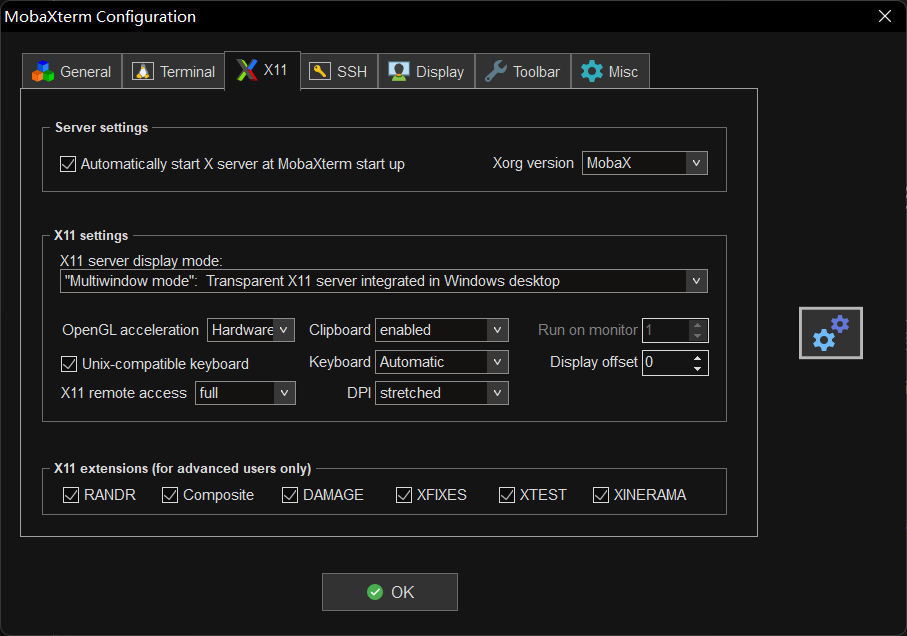
\includegraphics[width=\textwidth]{images/12.png}
        \caption{MobaXterm X11 Configuration.}
    \end{figure}
    Move the cursor on the icon of "X server", and you will see that it listens to all displays broadcasting \cite{mobaxtermdoc}:
    \begin{figure}[H]
        \centering
        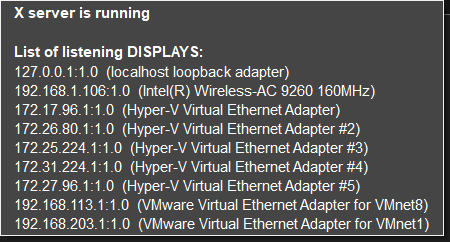
\includegraphics[width=\textwidth]{images/10.png}
        \caption{X server is running.}
    \end{figure}
    Also, check you have set up X11-forwarding and compression for command-line SSH:
    \begin{figure}[H]
        \centering
        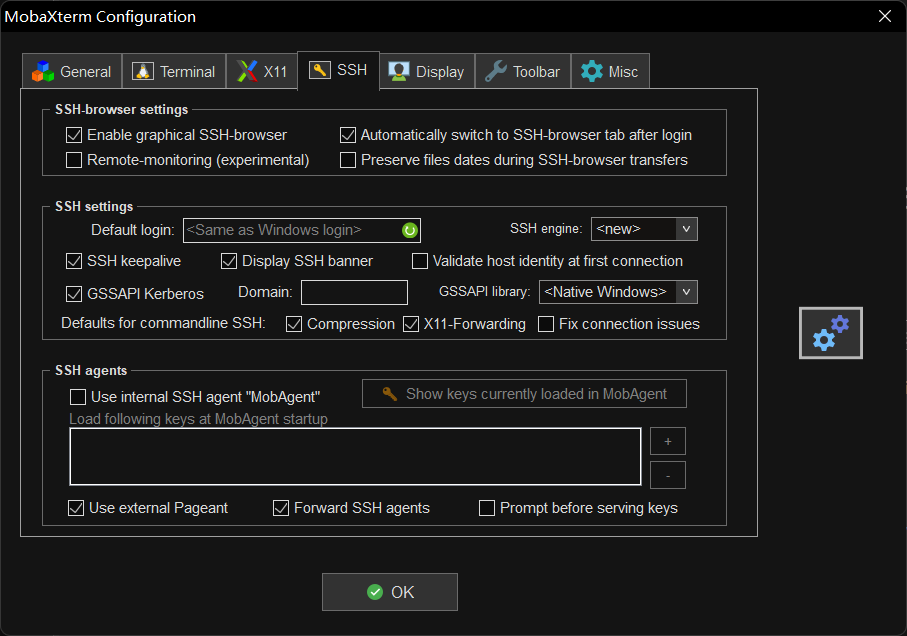
\includegraphics[width=\textwidth]{images/11.png}
        \caption{MobaXterm SSH Configuration.}
    \end{figure}
    \item You can run \texttt{echo \$DISPLAY} to check if your DISPLAY variable is automatically set to localhost:*.0 where * is 
a number. If not set, run \texttt{setenv DISPLAY localhost:*.0} to set. Note that the remote server is CentOS 6.10 Final and tcsh 6.17.00 Astron, so commands are different from Ubuntu Bash. Run graphical UI applications like \texttt{xclock} or \texttt{gedit} to test whether your X server works correctly. If you see the output
    \begin{minted}[breaklines]{text}
MoTTY X11 proxy: unable to connect to forwarded X server: Network error: Connection refused
Error: Can't open display: localhost:11.0
    \end{minted}
    go to Appendix: \ref{AMobaX}. If you see the output
    \begin{minted}[breaklines]{text}
Warning: Missing charsets in String to FontSet conversion
    \end{minted}
    Run \cite{lcctype}
    \begin{minted}[breaklines]{bash}
setenv LC_TYPE C
    \end{minted}
\end{enumerate}
MobaXterm is based on Cygwin technology using the MoTTY terminal. You can open the MobaXterm terminal from the Terminal tab->Open new tab or click the "+" button on the tab control bar. The bundled Cygwin system is CYGWIN\_NT-10.0-WOW i686 GNU/Linux. You can check the status of X server host by running \texttt{xhost} in the MobaXterm terminal. If it outputs like
\begin{minted}{text}
access control enabled, only authorized clients can connect
INET:Administrator
LOCAL:
\end{minted}
\begin{figure}[H]
    \centering
    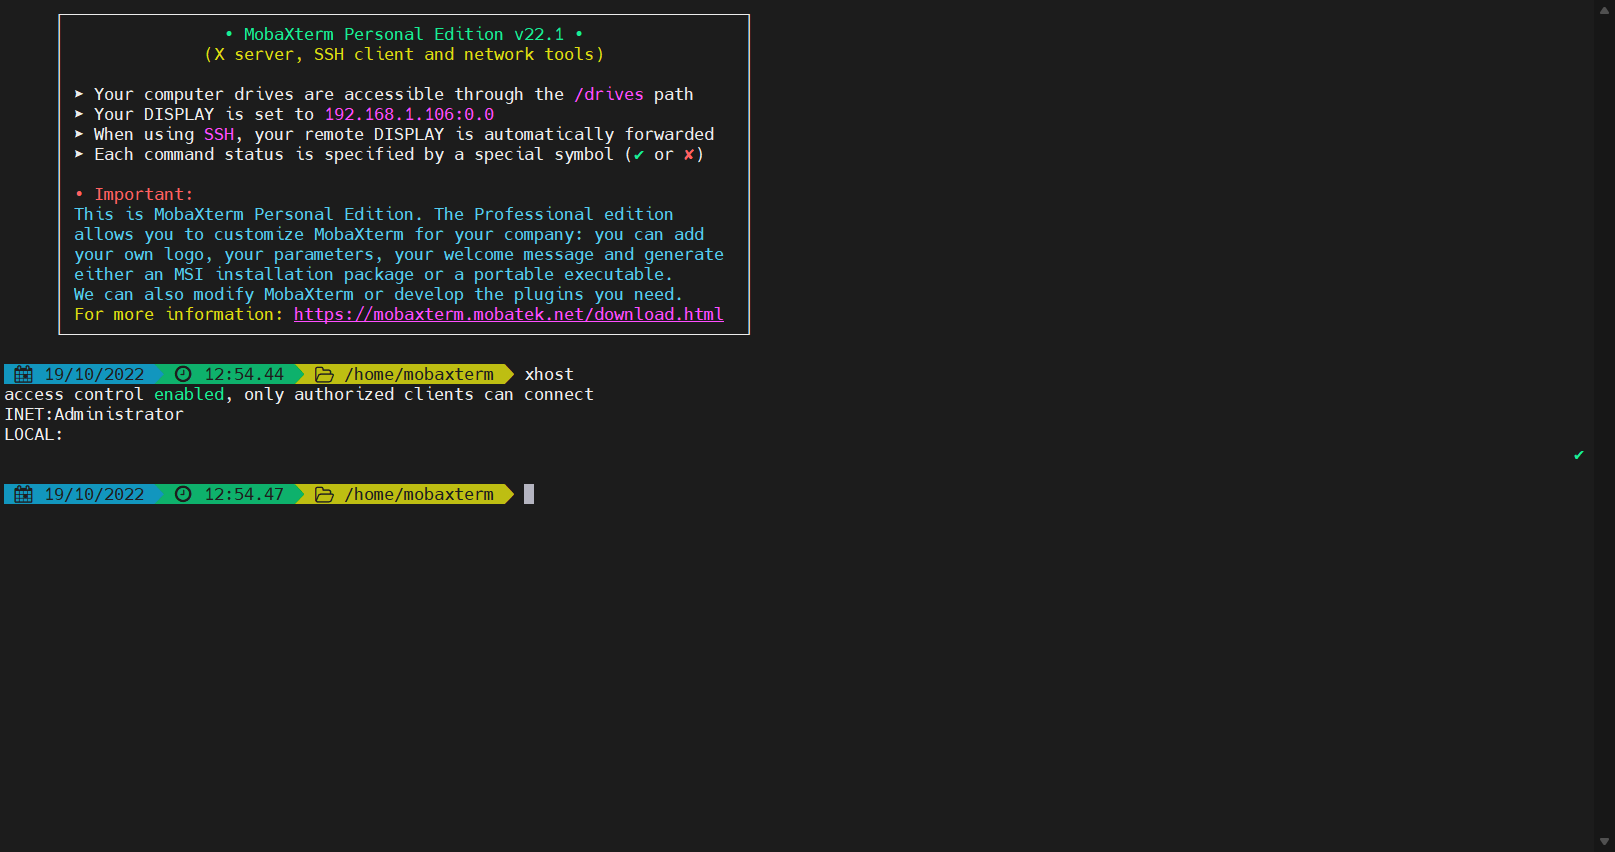
\includegraphics[width=\textwidth]{images/9.png}
    \caption{MobaXterm terminal and \texttt{xhost}.}
\end{figure}
Then everything is OK \cite{uppmax}.

The log file of MabaXterm can be viewed from the Help menu->View MobaXterm log file in C:/Users/<username>/AppData/Roaming/MobaXterm/slash/tmp/MobaXterm.log. Open Windows Settings->Update \& Security for Windows 10 or Privacy \& Security for Windows 11->Windows Security->Open Windows Security. In Windows Security, go to Firewall \& network protection, click "Allow an app through firewall", or go to Control Panel->System and Security->Windows Defender Firewall->Allowed apps, where you can allow apps to communicate through Windows Defender Firewall. If you want, you can click "Change settings" so that you can click the "Allow another app...(R)" button. Scroll down the list of allowed apps and features, find the item "xwin\_mobax.exe" and it is checked on both the Private column and the Public column. You can check the log file of MobaXterm X Server from C:/Users/<username>/AppData/Roaming/MobaXterm/slash/\\
var/log/xwin named as XWin.*.log and XWin.*.log.old.

Also, check your C:/Users/<username>/AppData/Roaming/MobaXterm/slash/etc/hosts file that it is symlinked to the Windows hosts by
\begin{minted}{text}
!<symlink>/drives/C/Windows/system32/drivers/etc/hosts
\end{minted}
and files like protocol, services, and networks are also symlinked to Windows' counterparts.

The XWin\_MobaX.exe is updated from CygWin's XWin.exe, so it also accepts arguments of XWin. The documentation of XWin is \cite{xwindoc}.
\subsubsection{Connect by PuTTY + VcXsrv}\label{S22}
There are two popular options for standalone X servers on Windows: Xming and VcXsrv. However, Xming is no longer purely free and open-source: its latest free release is Xming 6.9.0.31, released on May 4, 2007, on SourceForge \href{https://sourceforge.net/projects/xming/}{Xming X Server for Windows}. The newer releases require \textsterling10 donations to obtain from \href{http://www.straightrunning.com/XmingNotes/}{Xming X Server}. Thus, Xming is not recommended. Instead, VcXsrv is actively under development on SourceForge, freely and open source, so using VcXsrv is recommended.

For SSH client terminals, there are too many alternatives. For simplicity, you can just use PuTTY. You can also use other products like \href{https://www.vandyke.com/products/securecrt/}{SecureCRT}.
\begin{enumerate}
    \item Download and install \href{https://www.chiark.greenend.org.uk/~sgtatham/putty/latest.html}{PuTTY}.
    \item Download and install \href{https://sourceforge.net/projects/vcxsrv/files/latest/download}{VcXsrv Windows X Server}.
    \item After installation, you should find XLauch shortcuts; if not, go to the installation directory of VcXsrv and run \texttt{xlaunch.exe}.
    \item In the Display settings, select Multiple windows and leave the Display number as -1 (0 is also OK).
    \begin{figure}[H]
        \centering
        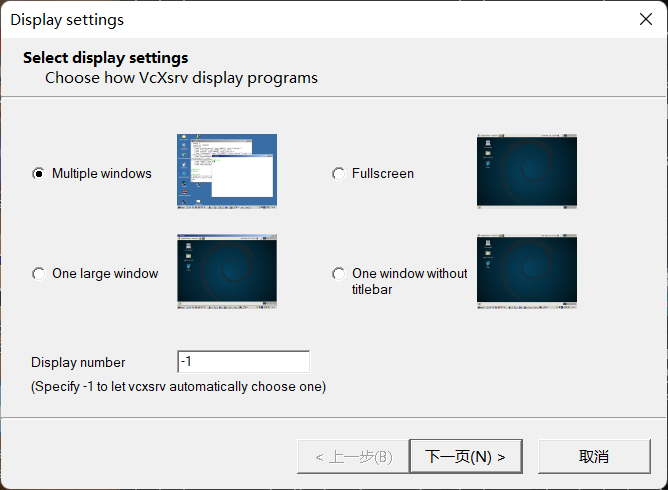
\includegraphics[width=0.85\textwidth]{images/1.png}
        \caption{VcXsrv XLaunch Display settings.}
    \end{figure}
    \item In the Client startup, select "Start no client".
    \begin{figure}[H]
        \centering
        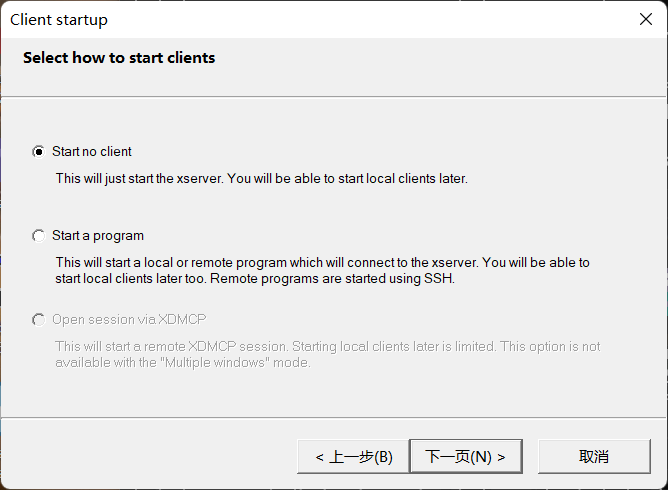
\includegraphics[width=0.85\textwidth]{images/2.png}
        \caption{VcXsrv XLaunch Client startup.}
    \end{figure}
    \item In the Extra settings, check "Clipboard", "Primary Selection", and "Native opengl". Generally, you do not need to check "Disable access control". Leave the Additional parameters for VcXsrv empty.
    \begin{figure}[H]
        \centering
        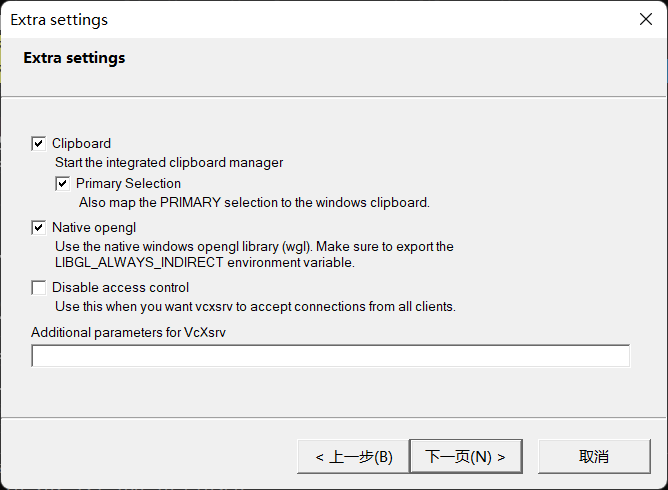
\includegraphics[width=0.75\textwidth]{images/3.png}
        \caption{VcXsrv XLaunch Extra settings.}
    \end{figure}
    \item In the Finish configuration, you can save the configuration for later use, but it is not necessary.
    \begin{figure}[H]
        \centering
        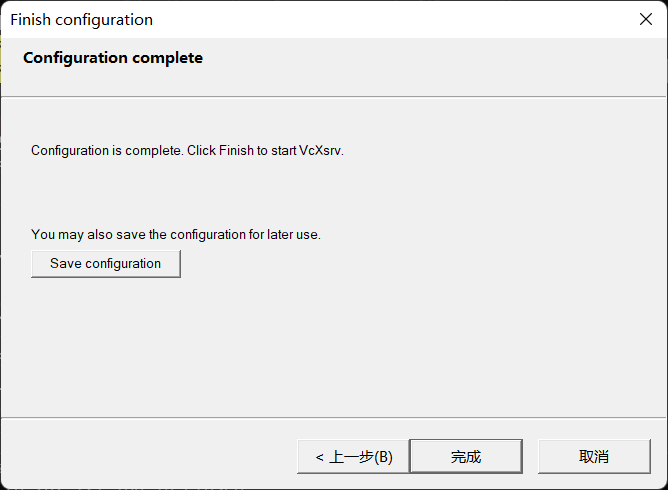
\includegraphics[width=0.75\textwidth]{images/4.png}
        \caption{VcXsrv XLaunch Finish configuration.}
    \end{figure}
    \item Make sure the icon of XLaunch keeps showing in the tray. If XLaunch exits silently, go to Appendix: \ref{AXLaunch}.
    \item Open PuTTY, then the PuTTY Configuration dialog will be opened. In the Category, select "Session". In the "Specify the destination you want to connect to" frame, fill in the Host Name (or IP address) and the Port. For the Connection type, select SSH. You can save the session in the "Load, save or delete a stored session" frame, and load the session from the Saved Sessions later.
    \item Go to Category->Connection->SSH->X11, in the X11 forwarding frame, check "Enable X11 forwarding". Select MIT-Magic-Cookie-1 as the Remote X11 authentication protocol. Generally, you can just leave X display location and X authority file for local display. But if needed, specify the X display location as ":0.0" or "127.0.0.1:0.0" or "localhost:0.0". Here, the first 0 is the display number, and the second 0 is the screen number. The X authority file for local display is \texttt{xauth.exe} under the installation directory of VcXsrv.
    \begin{figure}[H]
        \centering
        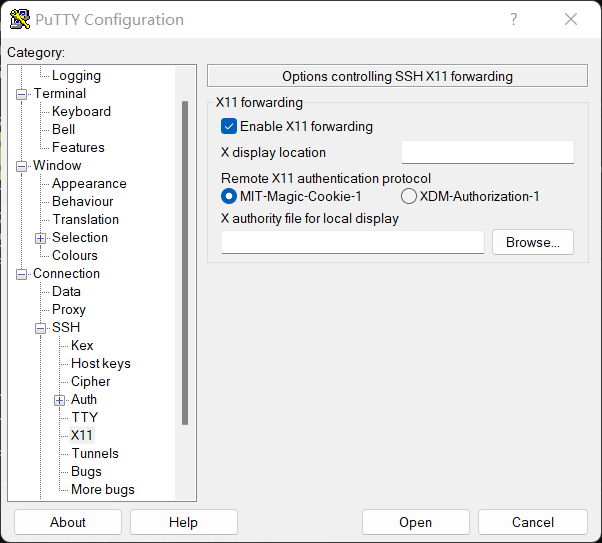
\includegraphics[width=\textwidth]{images/5.png}
        \caption{PuTTY X11 configuration.}
    \end{figure}
    \item Click "Open". In the PuTTY terminal, input your username and password as prompted. After you have done this, you can run graphical UI applications like \texttt{xclock} or \texttt{gedit} to test whether your X11 forwarding works well.
\end{enumerate}
The process for Xming and MobaXerm X Server is the same as above. Open MobaXterm X Server; then establish an SSH connection with X11 forwarding through PuTTY, you can also open X11-forwarded windows.
\subsubsection{Connect by Command Line + VcXsrv}\label{S23}
Still, download and install VcXsrv and run it first.

Following \cite{mslearnssh}, to install OpenSSH using PowerShell, run PowerShell as an Administrator. To make sure that OpenSSH is available, run the following cmdlet:
\begin{minted}[breaklines,linenos]{bat}
Get-WindowsCapability -Online | Where-Object Name -like 'OpenSSH*'
# Install the OpenSSH Client
Add-WindowsCapability -Online -Name OpenSSH.Client~~~~0.0.1.0
# Install the OpenSSH Server
Add-WindowsCapability -Online -Name OpenSSH.Server~~~~0.0.1.0
# Start the sshd service
Start-Service sshd
# OPTIONAL but recommended:
Set-Service -Name sshd -StartupType 'Automatic'
# Confirm the Firewall rule is configured. It should be created automatically by setup. Run the following to verify
if (!(Get-NetFirewallRule -Name "OpenSSH-Server-In-TCP" -ErrorAction
    SilentlyContinue | Select-Object Name, Enabled)) {
    Write-Output "Firewall Rule 'OpenSSH-Server-In-TCP' does not exist, creating it..."
    New-NetFirewallRule -Name 'OpenSSH-Server-In-TCP' -DisplayName 'OpenSSH Server (sshd)' -Enabled True -Direction Inbound -Protocol TCP -Action Allow -LocalPort 22
} else {
    Write-Output "Firewall rule 'OpenSSH-Server-In-TCP' has been created and exists."
}
\end{minted}
Alternatively, to install OpenSSH by GUI,
\begin{enumerate}
    \item Open Settings, select Apps, then select Optional Features.
    \item Scan the list to see if the OpenSSH is already installed. If not, at the top of the page, select Add a feature, then:
    \begin{itemize}
        \item Find OpenSSH Client, then select Install
        \item Find OpenSSH Server, then select Install
    \end{itemize}
    Once setup completes, return to Apps and Optional Features, and you should see OpenSSH listed.
\end{enumerate}
Installing OpenSSH Server will create and enable a firewall rule named OpenSSH-Server-In-TCP. This allows inbound SSH traffic on port 22. If this rule is not enabled and this port is not open, connections will be refused or reset.

\begin{itemize}
    \item Use Command Prompt (cmd.exe): Run
    \begin{minted}{bat}
set DISPLAY=localhost:0.0
ssh -Y <username>@<hostname> -p <port>
    \end{minted}
    \item Use Windows PowerShell (powershell.exe) or PowerShell (Core) (pwsh.exe): Run \cite{pwshx11}
    \begin{minted}{bat}
$env:DISPLAY='localhost:0.0'
ssh -Y <username>@<hostname> -p <port>
    \end{minted}
\end{itemize}
You can run CMD or PowerShell in (Windows) Terminal.

Please use the \texttt{-Y} argument. Usually, the command \texttt{ssh} is aliased by \texttt{ssh -X}. The \texttt{-X} argument is to enable X11 forwarding, but users with the ability to bypass file permissions on the remote host (for the user's X authorization database) can access the local X11 display through the forwarded connection, and an attacker may then be able to perform activities such as keystroke monitoring. Instead, \texttt{-Y} argument enables trusted X11 forwarding. Trusted X11 forwardings are not subjected to the X11 SECURITY extension controls \cite{sshman}. In \texttt{/etc/ssh/ssh\_config} on your server, the \texttt{ForwardX11Trusted} option has been set to "yes", so that remote X11 clients will have full access to the original X11 display \cite{sshconfigman}.
\begin{figure}[H]
    \centering
    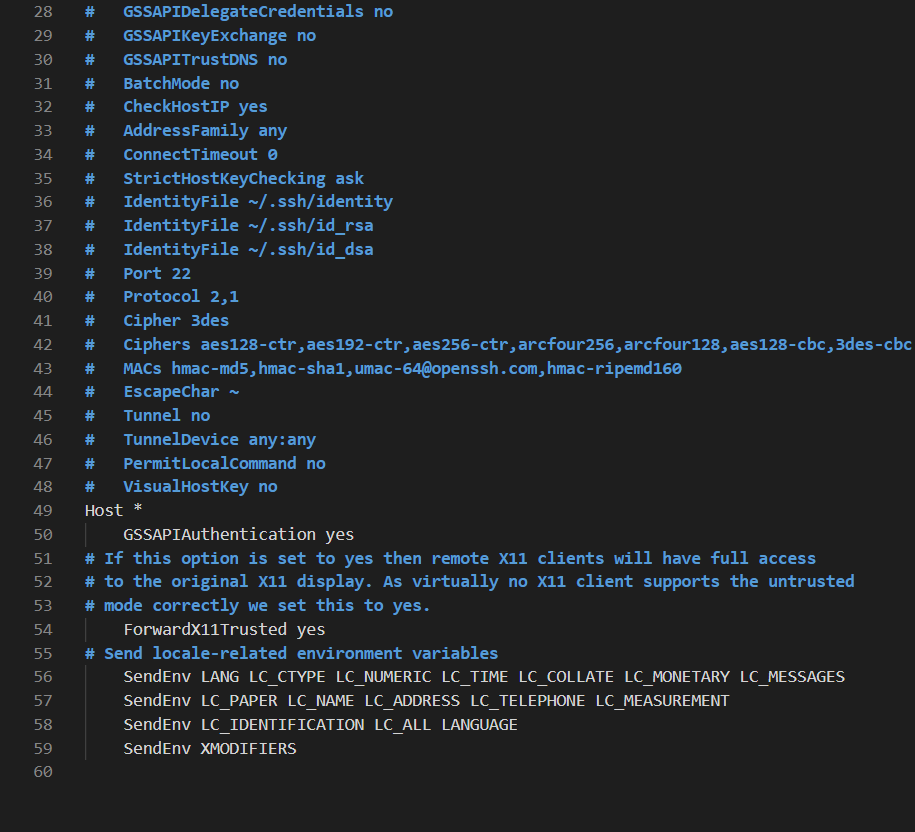
\includegraphics[width=0.7\textwidth]{images/6.png}
    \caption{\texttt{ssh\_config}.}
\end{figure}
\subsection{VNC connection}
\begin{enumerate}
    \item Open VMware Horizon Client and login \texttt{vdi.ji.sjtu.edu.cn}.
    \item Then, start the Student virtual machine through VMware Blast.
    \item Open the VNC Viewer. Enter the VNC Server address 10.11.13.66:6000.
    \begin{figure}[H]
        \centering
        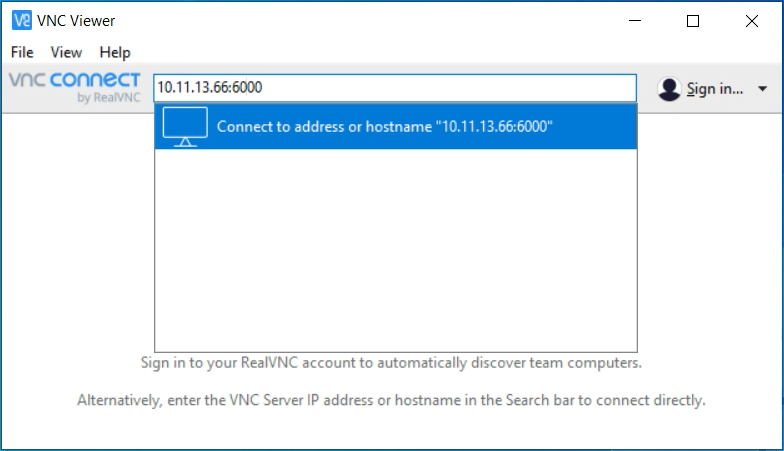
\includegraphics[width=0.8\textwidth]{images/7.png}
        \caption{VNC Viewer login.}
    \end{figure}
    \item In the Authentication dialog, enter your Username and Password for your SSH server and click OK.
    \begin{figure}[H]
        \centering
        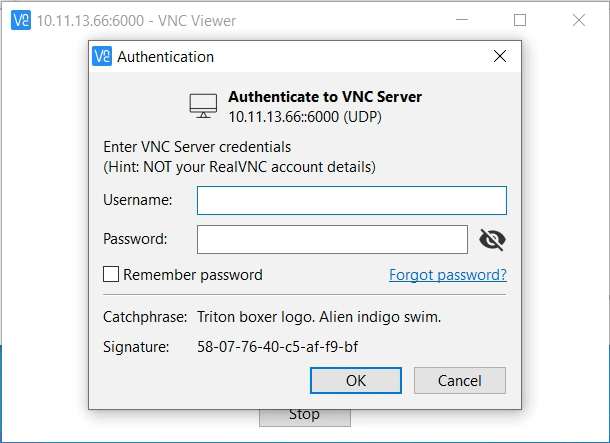
\includegraphics[width=0.8\textwidth]{images/8.png}
        \caption{VNC Viewer Authentication.}
    \end{figure}
    % \item You can access the Linux desktop now.
\end{enumerate}
\subsection{TENEX C Shell Run Commands}
The server uses TENEX C Shell (tcsh), a Unix shell based on and backward compatible with the C shell (csh). It is essentially the C shell with programmable command-line completion, command-line editing, and a few other features. Unlike the other common shells, functions cannot be defined in a tcsh script, and the user must use aliases instead (as in csh). It is the native root shell for BSD-based systems such as FreeBSD. The Run Commands (RC) file \texttt{.cshrc} is not complex. It sets several variables which are not used often. It first sources \texttt{apps/env/modules.csh} which sources \texttt{/apps/systools/modules-4.7.1/init/tcsh} (here tcsh and csh files are the same) and \texttt{apps/env/cshrc.alias} which set aliases, \texttt{module load} python and htop, and set \texttt{MODULEPATH} environment. Then it sources the seven sub csh files for ANSYS, KeySight, Cadence, Synopsys, Mentor, Mathworks, and MC2 software. In the end, it appends the paths of all the available software to the system PATH variable.

The sub csh files of EDA software set license files and \texttt{module load} the tools of the software.

In this lab, we will use Synopsys Design Compiler Version R-2020.09-SP3 for linux64, which has a much better graphical user interface, so change the corresponding entry in the PATH to \texttt{/apps/synopsys/syn-2020.09/bin}.

\section{Introduction to Synopsys EDKs}
\subsection{Overview}
In this lab, you will use Synopsys 90nm Process Design Kit (PDK) or educational purpose 32/28nm Generic Library as a part of Synopsys Educational Design Kits (EDKs) under /home/pdk/synopsys\_edk/edk90/synopsys\_design\_flow\_using\_90nm\_library and /home/pdk/synopsys\_edk/edk32. The directory structure of Synopsys 90nm PDK is
\begin{itemize}
    \item dc - directory for logic synthesis
    \item fm - directory for formal verification
    \item hercules - directory for post-layout DRC, LVS checks
    \item icc - directory for physical synthesis
    \item models - directory for technology files for standard cells in Liberty syntax
    \item ptpx - directory for power analysis
    \item ref - all needed information for physical synthesis
    \item src - RTL directory
    \item sta - directory for static timing analysis
    \item starrc - directory for post-layout parasitic extraction
    \item tmax - directory for ATPG generation
    \item vcs -directory for functional verification
    \item verilog -  Verilog codes of library cells
\end{itemize}
A process design kit (PDK) is a set of files used within the semiconductor industry to model a fabrication process for the design tools used to design an integrated circuit. The PDK is created by the foundry defining a certain technology variation for their processes. It is then passed to their customers to use in the design process. The customers may enhance the PDK, tailoring it to their specific design styles and markets. The designers use the PDK to design, simulate, draw and verify the design before handing the design back to the foundry to produce chips. The data in the PDK is specific to the foundry's process variation and is chosen early in the design process, influenced by the market requirements for the chip. An accurate PDK will increase the chances of first-pass successful silicon.

\subsection{Theoretical parts}
\subsubsection{Design Compiler}
\begin{enumerate}
    \item Design Compiler optimizes designs to provide the smallest and fastest logical representation of a given function. It comprises tools that synthesize HDL designs into optimized technology-dependent, gate-level designs. It supports a wide range of flat and hierarchical design styles and can optimize both combinational and sequential designs for speed, area, and power.
    \item DC uses information from the setup file for normal operation. In this file, DC searches technology libraries in search\_path. In the setup file target\_library, link\_library, and synthetic library are technology files in liberty syntax. DC used the mentioned files while transferring the RTL design to the gate-level design. The link and target libraries are technology libraries that define the semiconductor vendor’s set of cells and related information, such as cell names, cell pin names, delay arcs, pin loading, design rules, and operating conditions. Here variable lib\_path can be found, which shows the path to milkyway reference library for the physical synthesis tool. By means of using \texttt{set mw\_reference\_library} command, reference milkyway library can be given to the physical synthesis tool.
    \item The first stage of the synthesis process is to analyze and elaborate RTL. In elab.tcl, command \texttt{define\_design\_lib} is used to show the path to the design library, which contains the analyzed form of RTL. In this script, the source command is used to execute the setup script. After sourcing the setup file, the design can be elaborated. For this command, elaborate is used. Then, the design is uniquified. Afterward, the write command is used to save the elaborated design.
    \item In order to perform the next steps, compile.tcl is used. Here first setup file is sourced again. Then, design is read using \texttt{read\_ddc} command. After reading the design, the current design must be set for which \texttt{current\_design} command is used. Then it is necessary to link the design to its references. Link command is used. Design constraints are given in another file which is read using the source command. Here gate level netlist with GTECH gates becomes a gate-level netlist with gates from a given technology library by compile command. To see the results, different types of write and report commands are used.
\end{enumerate}
\subsubsection{Formality}
\begin{enumerate}
    \item Formality is an application that uses formal techniques to prove or disprove the functional equivalence of two designs or two cell libraries. For example, users can use Formality to compare a gate-level netlist to its register transfer level (RTL) source or to a modified version of that gate-level netlist. After the comparison, Formality reports whether the two designs or cell libraries are functionally equivalent.
    \item Formality creates FM\_WORK directory upon invocation. It contains containers and shared technology libraries.
    \item A container is a complete, self-contained space into which Formality reads designs. It is typical for one container to hold the reference design while another holds the implementation design. In general, a user does not need to concern himself with containers. Design is loaded either as a reference or implementation.
    \begin{itemize}
        \item \texttt{read\_vhdl –c ref Ref\_file\_path\_name} – the mentioned file is read in container as a reference
        \item \texttt{read\_verilog –c impl Impl\_file\_path\_name} – the mentioned file is read in container as implementation
        \item \texttt{set\_top ref: /*/Top\_design} - sets the top-level design for the reference
        \item \texttt{set\_top impl: /*/Top\_design} - sets the top-level design for the implementation
        \item \texttt{read\_db –c impl lib\_db\_file –technology\_library} – loads in container technology library for implementation
        \item \texttt{report\_containers} - Produces a list of containers
        \item \texttt{current\_container} – sets or gets a current container
        \item \texttt{cputime} - Returns the CPU time used by the Formality shell
        \item \texttt{verify ref: /WORK/top\_design impl:/WORK/top\_design} – verifies reference and implementation design equivalency
        \item \texttt{report\_status} – reports verification results
    \end{itemize}
\end{enumerate}
\subsubsection{IC Compiler}
\begin{enumerate}
    \item IC Compiler is a single, convergent netlist-to-GDSII or netlist-to-clock-tree-synthesis design tool for chip designers developing very deep submicron designs. Gate-level netlist, a detailed floorplan, timing constraints, physical and timing libraries, and foundry-process data are given to its input, and it generates either a GDSII-format file of the layout or a Design Exchange Format (DEF) file of placed netlist data ready for a third-party router as an output. IC Compiler can also output the design as a binary Synopsys Milkyway database at any time for use with other Synopsys tools based on Milkyway or as ASCII files (Verilog, DEF, and timing constraints) for use with not Synopsys tools.
    \item ICC uses information from the setup file for normal operation. In this file, search\_path is mentioned where ICC searches technology libraries. In the setup file target\_library, link\_library and synthetic library are technology files in liberty syntax. The link and target libraries are technology libraries that define the semiconductor vendor’s set of cells and related information, such as cell names, cell pin names, delay arcs, pinloading, design rules, and operating conditions. Here variable \texttt{lib\_path} can be found, which shows the path to milkyway reference library. By means of using \texttt{set mw\_reference\_library} command, reference milkyway library is given to ICC.
    \item Other design steps are done using synthesis.tcl script.
    \begin{enumerate}
        \item Here first setup file is sourced for which source command is used.
        \item Then in order to start physical synthesis, it is necessary to create milkyway library with \texttt{create\_mw\_lib} command. These command options with their descriptions are given below:\\
        library name – name of created library\\
        -tech techfile\_name.tf – give technology file\\
        -mw\_reference\_library "\$ref\_lib\_name" – give milkyway reference library
        \item After creating the library, it is necessary to open the library. In order to do this, \texttt{open\_mw\_lib} command is used.
        \item Then, the design obtained by DC must be read. To read the design, \texttt{read\_ddc} command is used.
        \item After reading the design, the floorplan must be done. In order to do this,\\
        \texttt{initialize\_floorplan} command with all necessary options is used.
        \item Then power and ground connection must be done with \texttt{derive\_pg\_connection} command.
        \item The next step in the physical synthesis process is to create rectangular rings for power and ground supplies. In order to do this, \texttt{create\_rectangular\_rings} command with all options is used.
        \item To create power and ground straps \texttt{create\_power\_straps} command is used.
        \item Afterwards FP placement (create\_fp\_placement) is done.
        \item Then prerouting of standard cells follows (preroute\_standard\_cells).
        \item Afterwards, placement is done (place\_opt).
        \item Final steps in the physical synthesis process are CTS (clock\_opt) and routing (route\_opt).
    \end{enumerate}
\end{enumerate}
\subsubsection{Hercules}
\begin{enumerate}
    \item Hercules can verify layout Design Rule Checks (DRC), perform Electrical Rule Checks (ERC), extract layout structures, and compare them to an original design netlist by using the Layout versus Schematic (LVS) application and generate or modify data for mask preparation. The hierarchical checking of algorithms makes Hercules particularly well-suited for large and complex IC verification.
    \item While working with Hercules user uses Runset files. Runset files are ASCII (text) files containing instructions for determining where Hercules gets its files and how it runs. The Runset file contains the following sections.
    \begin{itemize}
        \item Runset Header information
        \item Runset options
        \item Preprocessing options
        \item Layer assignments
        \item SNAP command
        \item GRID checks
        \item DRC checks
    \end{itemize}
    \item DRC Runset Header information section is defined by the keyword HEADER, found in the left margin of the file. The HEADER section contains variables that define where Hercules can find the layout libraries and other input files. The HEADER section also contains information about where to write intermediate processing files and output files.
    \begin{itemize}
        \item The INLIB variable tells Hercules the name of the input library that the user wants to check. If the user uses GDSII formatted data, the INLIB line needs to specify a complete path and GDSII file name.
        \item The BLOCK tells Hercules the name of the top-level input structure which the user wishes to verify.
        \item The OUTLIB setting tells Hercules the name of the output library, which contains all the permanent output layers (created by Hercules), error output, and newly-created graphical layers.
        \item The OUTPUT\_BLOCK setting tells Hercules what to call the top-level output structure that holds all of your error hierarchy and permanent output layer placements.
        \item The GROUP\_DIR setting tells Hercules where to place all the group files it temporarily creates. Group files contain the data on which Hercules works during runset execution.
    \end{itemize}
    \item DRC Runset OPTIONS section allows specifying global assignments for various Hercules processes. Hercules also has a DRC\_OPTIONS section. All variables in the DRC\_OPTIONS section may also be placed in the OPTIONS section.
    \item The PREPROCESS\_OPTIONS section allows users to specify the output of information and the setting of path grid checking options. Users can set options for increased information in the block. LAYOUT\_ERRORS file and the tree files. Users can also set options for path grid checking, which is done when the layers are read during the ASSIGN section. For example, setting the CHECK\_PATH\_90 option to FALSE allows users to have 45-degree path data in design.
    \item The ASSIGN section assigns names to the database layers found in the design.
    \item The SNAP command section forces data to conform to a grid resolution during a run.
    \item The GRID\_CHECK command performs grid checking after group file creation and appears in the runset after the ASSIGN section.
    \item DRC Checks - here user writes commands to check DRC violations. For the results, see Block\_name.LAYOUT\_ERRORS
    \item LAYOUT\_PATH, INLIB, BLOCK, OUTLIB, FORMAT, and GROUP\_DIR variables in LVS runset files HEADER are the same as in DRC runset file. Four variables in HEADER, which are not the same as in DRC runset HEADER, are given below.
    \begin{itemize}
        \item COMPARE\_DIR - This setting tells Hercules where to place all the COMPARE output files it temporarily or permanently creates. The default value for the COMPARE\_DIR variable is run\_details/compare/.
        \item EQUIVALENCE - This variable specifies the location and name of the equivalence file. The equivalence file is a comparison input file that lists the structures to be compared. It is generally referred to as the EQUIV file.
        \item SCHEMATIC - This variable is set to the file name, including the path, of the schematic netlist file. This variable is required to execute a Hercules LVS run. If a user does not specify this file, or if Hercules cannot find the file user specifies, the Hercules job terminates with an error indicating that the schematic file is not specified or that Hercules cannot open the schematic netlist for reading.
        \item SCHEMATIC\_FORMAT - This variable is set to the format type of the input schematic netlist. Hercules supports CDL, Hercules, SPICE, EDIF, EDIF3, VERILOG, and SILOS. This variable is required if the specified input schematic netlist is not in the Hercules format. If this format is set to something other than Hercules, Hercules calls NetTran, the netlist translation utility.
    \end{itemize}
    For results, see Block\_name.LVS\_ERRORS.
\end{enumerate}
\subsubsection{PrimeTime}
\begin{enumerate}
    \item PrimeTime is a full-chip, gate-level static timing analysis tool that is an essential part of the design and analysis flow for today’s large chip designs. PrimeTime exhaustively validates the timing performance of a design by checking all possible paths for timing violations without using logic simulation or test vectors.\\
    PrimeTime fits ideally into the Synopsys physical synthesis flow because it uses many of the same libraries, databases, and commands as other Synopsys tools such as Design Compiler. It can also operate as a stand-alone static timing analyzer in other design flows. It accepts design information in a wide range of industry-standard formats, including gate-level netlists in .db, Verilog, and VHDL formats; delay information in Standard Delay Format (SDF); parasitic data in Reduced Standard Parasitic Format (RSPF), Detailed Standard Parasitic Format (DSPF), Standard Parasitic Exchange Format (SPEF), and Synopsys Binary Parasitic Format (SBPF) formats and timing constraints in Synopsys Design Constraints (SDC) format.\\
    If PrimeTime finds any timing violations, the design needs to be resynthesized using new timing constraints (generated by PrimeTime) to fix the conditions that are causing the timing errors.\\
    The GUI offers some visual analysis capabilities that are not available in pt\_shell. For example, users can view schematics of the design, display clock waveforms, and generate histograms of analysis results, such as path slack, net capacitance, and bottleneck cost. The console window within the top-level window lets users enter commands and view the text response, just like pt\_shell.
    \item The first step is to read the gate-level design description and associated technology library information. PrimeTime accepts design descriptions and library information in .db format and .ddc and gate-level netlists in Verilog and VHDL formats. The corresponding commands for reading design files are read\_db, read\_ddc, and read\_verilog, read\_vhdl.\\
    After reading a set of hierarchical design files, the link\_design command resolves all references between different modules in the hierarchy and builds an internal representation of the design for timing analysis.\\
    To back-annotate the design with parasitic capacitance and resistance information, the read\_parasitics command is used. PrimeTime accepts detailed parasitic data in RSPF, DSPF, SPEF, and SBPF formats.
    \item These are some of the more common report commands:
    \begin{itemize}
        \item \texttt{report\_port} - Lists the ports and shows port information such as the direction, pin capacitance, wire capacitance, input delay, output delay, related clock, design rules, and wire load information.
        \item \texttt{report\_clock} - Generates a report on the clocks defined for the design, showing for each clock the name, period, rise and fall times, and timing characteristics such as latency and uncertainty.
        \item The \texttt{report\_timing} command is perhaps the most flexible and powerful PrimeTime analysis command. It provides general or more information about the timing of the whole design, a group of paths, or an individual path. The command options let users specify the types of paths reported, the scope of the design to search for the specified paths, and the type of information included in the path reports.
        \item The \texttt{report\_constraint} command reports the results of constraint checking done by PrimeTime. Users can obtain information such as the location of the worst violation, the amount by which the constraint is met or violated, and the calculation of the delays used for checking the constraint.
    \end{itemize}
\end{enumerate}
\subsubsection{PrimeTimePX}
\begin{enumerate}
    \item PrimeTime PX is an add-on feature to PrimeTime that accurately analyzes the power dissipation of cell-based designs. It is intended as an advanced solution for ASIC and structured custom circuit designers who are developing products for power-critical applications such as portable computing and telecommunications. PrimeTime PX builds a detailed power profile of the design based on the circuit connectivity, the switching activity, the net capacitance, and the cell-level power behavior data in the Synopsys database format (.db) library, which can be either a nonlinear power model (NLPM) or a Composite Current Source (CCS) library. It then calculates the power behavior for a circuit at the cell level and reports the power consumption at the chip, block, and cell levels. PrimeTime PX supports a gate-level netlist only.
    \item Set the power\_enable\_analysis variable to true to enable power analysis and see power data. The default value of this variable is false. If a user does not set this variable to true, he cannot see power data. A PrimeTime PX license is required to use this variable.\\
    Power analysis mode can be selected by using the power\_analysis\_mode variable. The syntax of this variable is as follows:\\
    \texttt{set power\_analysis\_mode averaged | time\_based}\\
    This variable must be set before using any of the power commands. If this variable is not set, PrimeTime PX, by default, performs averaged power analysis.\\
    The tool supports netlists in Verilog, VHDL, EDIF, .db, .ddc, and Milkyway formats. The technology library must be in the .db (Synopsys database) format. Both NLPM and CCS libraries are supported. \texttt{Read\_verilog} command can be used to read the design.\\
    In order to read the VCD file that contains the switching activity information read\_vcd command can be used. The \texttt{-rtl} option of the \texttt{read\_vcd} command is used to specify that the VCD is generated from an RTL simulation. If the VCD file is generated from a zero-delay simulation, the \texttt{-zero\_delay} option is used. When neither option is specified, the tool assumes that the file is a gate-level VCD file.\\
    Power analysis is triggered consistently for the various power analysis modes during the execution of the update\_power command. After the analysis, the \texttt{update\_power} command generates the power data.\\
    In order to generate an averaged or time-based power report that contains the power consumption for the design \texttt{report\_power} command can be used.
\end{enumerate}
\subsubsection{TetraMAX}
\begin{enumerate}
    \item TetraMAX is a high-speed, high-capacity automatic test pattern generation (ATPG) tool. It can generate test patterns that maximize test coverage while using a minimum number of test vectors for a wide variety of design types and design flows. It is well suited for designs of all sizes up to millions of gates.
    \item \texttt{read\_netlist} command is used to read the design. Option delete is used to clear in-memory designs and switch to new designs. \texttt{read\_netlist} command with option \texttt{–library} is used to read the library models. Building the ATPG design model takes the parts of the design which are to be part of the ATPG process, removes the hierarchy, and puts them into an in-memory image that TetraMAX can use. Design building is done by means of using \texttt{run\_build\_model} command. If design references undefined modules, TetraMAX sends error messages during execution of \texttt{run\_build\_model}. To identify all currently referenced modules, users can use the Netlist > Report Modules menu command or enter the \texttt{report\_modules -undefined} command. In order to perform DRC from the command line, \texttt{run\_drc} command can be used. Users can write out a template STIL file at any point after executing a \texttt{run\_build\_model}l command. To do so, the \texttt{write\_drc\_file} command or the Write tab in the DRC dialog box can be used. User can initialize the fault list for all faults using the \texttt{add\_faults -all} command. Some violation IDs show an abort indicator suffix, which appears as Z7-12.A or Z6-3 (Abort). This means that the ATPG analysis of the violation was aborted. In such cases, users might want to increase the ATP abort limit. Users can specify the pattern generation effort and other ATPG settings using the Run ATPG dialog box or can use the \texttt{set\_atpg} command at the command line. To run ATPG from the command line, the \texttt{run\_atpg} command is entered. User can generate a fault summary report using the \texttt{report\_summaries} or \texttt{report\_fault} command. In order to write test patterns from the command line \texttt{write\_patterns} command can be used.
\end{enumerate}
\subsubsection{VCS}
\begin{enumerate}
    \item VCS is a high-performance, high-capacity Verilog simulator that incorporates advanced, high-level abstraction verification technologies into a single open native platform. VCS enables analyzing, compiling, and simulating Verilog design descriptions. It also provides users with a set of simulation and debugging features to validate the design. These features provide capabilities for source-level debugging and simulation result viewing. VCS supports all levels of design descriptions but is optimized for the behavioral and register transfer levels.
    \item To create an executable named simv by default, the following VCS command line is used:\\
    vcs source\_file options. Here source\_file is .v file of a design that needs verification and testbench files. Some options are described below:
    \begin{itemize}
        \item -f filename-- Specifies a file name that contains a list of absolute path names for Verilog source files and compile-time options.
        \item -R--Runs the executable file immediately after VCS links it together. Any runtime option can be added to the VCS command line.
        \item -RI --Compiles model for interactive use, invokes the VirSim graphical user interface immediately after compilation, and pauses simulation at time zero.
        \item +v2k--Enables language features in the IEEE 1364-2001 standard.
        \item -v filename--Specifies a Verilog library file, in which VCS looks for the modules and UDP instances that are instantiated, but not defined, in the source code.
        \item +tetramax--Enables simulation of TetraMAX’s testbench in zero delay mode.
    \end{itemize}
\end{enumerate}
\subsubsection{StarRC}
StarRC is a software tool that extracts parasitics from connected databases that represent IC layout designs.

StarRC can be used to generate netlists to conduct timing, clock, noise, or power analysis.

Users can also extract parasitics like resistors, capacitors, and inductors from a layout design database.

(*.nxtgrd) is a database containing capacitance, resistance, and layer information, which can be encrypted. StarRC uses this output database (.nxtgrd file) to calculate the parasitics of the actual layout by pattern matching.

The mapping file, which maps the database layer to the tcad\_grd layer, is needed for every StarRC run. The mapping file can be written manually or by using the StarRC GUI. Mapping multiple database layers to a single process layer is valid, but the reverse is prohibited. Each logically connected database layer must be mapped in this file, even if the layer is derived or used only for intermediate connections with no real physical significance. In LEF/DEF flows, this means that each layer defined in the technology LEF file must be mapped (including VIAs).

For extraction, StarRC also uses .tf.

After extraction user gets extraction netlist in .spf format.

\subsection{Design process}
The overview of the design process is
\begin{enumerate}
    \item Logical synthesis in dc.
    \begin{enumerate}
        \item Edit the technology-specific file to use the library\\
        Also edit the clock frequency targets dc/scripts/setup.tcl.
        \item Invoke DC.
        \item Elaborate the design\\
        For this use ./scripts/elab.tcl.
        \item Synthesis of the design\\
        For this use ./scripts/compile.tcl\\
        Reports: ./reports/*\\
        DDC netlist: ./db/TOPDESIGN.ddc
    \end{enumerate}
    Analyze the results (reports to \texttt{backend} and \texttt{db} directories)
    \item Formal verification in fm.\\
    fm\_comp.scr.gate: This script is used to make a formal comparison between the RTL and gate-level netlist. 
    
    Procedure:\\
    run\_fm.gate script is provided to set up environment variables for the fm\_comp.scr.gate script.
    
    Usage:\\
    run\_fm.gate <src path> <library file> <netlist file> <dwroot path>
    
     <src path>     path to src directory. Under this directory, the RTL and the memory\_models directories must be present.
    
     <library file> this specifies the absolute or relative path to the db file of the library (do not use pg pin syntax library)
    
     <netlist file> this specifies the absolute or relative path to the .db,.ddc, or .v file of the gate-level netlist
    
     <dwroot path>  path to installation of Synopsys DesignWare
    
    Analyze the results (logs and reports directories)
    \item Physical analysis in icc.
    \begin{enumerate}
        \item Invoke ICC.
        \item Run script ./scripts/physical.tcl.
        \item Write GDS and .v from ICC to directory ../hercules (use information from write\_verilog\_write\_gds.txt).
    \end{enumerate}
    Analyze the results (spef and Milkyway library PARSER\_ICC directory).
    \item Post-layout DRC, LVS checks in Hercules.
    \begin{enumerate}
        \item Transfer Verilog from ICC to sp (use ./verilogtosp).
        \item Copy GDS and sp to ./DRC for DRC and ./LVS for LVS.
        \item Move to directory ./DRC for drc.
        \begin{enumerate}
            \item Invoke Hercules.
            \item Run script rules.drc.9m\_saed (use Hercules rules.drc.9m\_saed).
        \end{enumerate}
        Analyze the results (PARSER.LAYOUT\_ERRORS file).
        \item Move to directory ./LVS for lvs.
        \begin{enumerate}
            \item Invoke Hercules.
            \item Run script rules.drc.9m\_saed (use Hercules rules.drc.9m\_saed).
        \end{enumerate}
        Analyze the results (PARSER.LAYOUT\_ERRORS and PARSER.LVS\_ERRORS files).
    \end{enumerate}
    \item Static timing analysis in sta. The scripts provided allow users to run static timing at many different stages. run\_sta shell script is provided to enable the different options for running static timing.\\
    run\_sta.csh Switch Usage: 
      -netlist [path to netlist]        : Path+filename of netlist to time
      -speed [WC|BC|BC\_WC]             : operating condition, (default best\_case/worst\_case analysis if done)
      -spef [path]                      : Path+filename of spef file
      -dspf [path]                      : Path+filename of dspf file
      -load [path]                      : Path+filename of load file
      -sdf  [path]                      : Path+filename of sdf file
      -clk\_tree                        : post clock tree timing, otherwise ideal clocks are used
      -duty [45|50|55]                  : Clock duty cycle 45/55 or 50/50 (default) or 55/45
      -mode [sync|syncbypass|capture|shift] : mode of operation (default = sync)
      -write\_sdf                       : sdf file will be written out
      -no\_reports                      : indicates interactive mode without generation all the timing reports
      -report\_dir [sub-dir name]       : Sub Directory to write timing reports i.e. ./reports/[sub-dir] (default = ./reports)
    
    The following explains each switch and describes when it is appropriate to use them.
    Switch Usage
    
      -netlist [path to netlist]: This switch is required and points to the Verilog, VHDL,  or .db gate-level netlist that needs to be timed.
    
      -speed [WC|BC|BC\_WC]: This switch is optional. The default is to run PrimeTime in best case / worst case mode, meaning that setup times are checked with respect to the worst case library and hold times are checked with respect to the best case library.
    
         WC: specifies that setup and hold times are checked with respect to the worst-case library
         BC: specifies that setup and hold times are checked with respect to the best-case library
    
         NOTE: The libraries are defined in the ../dc/scripts/setup.tcl
     
      -spef [path]: This switch must provide the path and filename to a SPEF parasitic file.
    
         Use 2.5D Parasitic Extraction data as soon as possible to provide the most accurate timing results. Note: Even though the Physical Compiler scripts write out a spef file, it is not meant for timing analysis; the Physical Compiler is not an extraction tool.
    
      -dspf [path]: This switch must provide the path and filename to a DSPF parasitic file.
    
      -load [path]: This switch must provide the path and filename to a Load parasitic file.
    
      -sdf [path]: This switch must provide the path and filename to an SDF parasitic file.
    
      -clk\_tree: This switch should only be used if clock trees have been added to your design. Specifying this switch removes the ideal attributes on the clocks. Also, detailed clock reports are generated when this switch is used.
    
      -duty [45|50|55]: This switch specifies the duty cycle of the clock. The default is 50%.
    
      -mode [sync|syncbypass|capture|shift] : The default is to run timing analysis in functional mode. shift times scan chain shift capture times scan chain capture logic
    
      -write\_sdf: This switch is optional. When used, an SDF file is generated.
     
      -no\_reports: This switch should only be used if you want to run PrimeTime interactively. With this switch active, the design will be setup with the constraints applied, and the pt\_shell prompt will be available for interactive use.
    
      -report\_dir [sub-dir]: path to a directory where you want the timing reports to be written to.\\
         The default is ./reports. If the directory doesn't exist, it is created.\\
         If a sub-dir is specified, the reports are written to ./reports/[sub-dir].\\
         If a sub-dir is specified, the logs are written to ./logs/[sub-dir].\\
    Currently, the script generates timing models by default, in case timing models are not required, pls set the gen\_model variable to false.
    
    Analyze the results (logs and reports directories).
    \item Power analysis in ptpx.\\
    The Power Analysis is run using the Prime Time tool. This is moved from Prime Power. The current version supports two types of Analysis
    \begin{enumerate}
        \item Vectorless Analysis
        \item VCD Based Analysis
    \end{enumerate}
    Flow:\\
    The power analysis is run with the following command,
    \begin{minted}{bash}
run_ptpx.tcl -netlist <path_to_netlist_file> \
             -para <path_to_parasitics_file> \
             -sa vcd -sa_file <path_to_VCD_file>
    \end{minted}
    Options:\\
    \texttt{-report\_dir <path\_to\_report\_dir>} : The Power Analysis reports are stored in this path. By default, the reports are stored in the ./reports directory

    \texttt{-extn [tag]} : To differentiate between different run, this option can be used.

    Analyze the results (logs and reports directories.
    \item ATPG generation in tmax.\\
    PARSER\_tmax.scr: This script is used for ATPG based on the fast sequential methodology of the TetraMax.\\
    Assumptions:
    \begin{itemize}
        \item You have access to TetraMax.
        \item Your environment should have the \$SYNOPSYS path set to point to the Synopsys tool installation directory.
        \item You have Verilog simulations libraries for your technology
    \end{itemize}
    Procedure:\\
    The run\_tmax.csh shell script is provided to set up the three environment variables that are required by the Tetramax script: The path to the netlist file, the path to the Verilog technology, the simulation library.\\
    Example:
    \begin{minted}{bash}
run_tmax.csh -netlist <Path + filename to netlist>
             -tech_lib ../verilog/ALL.v
    \end{minted}
    Analyze the results (logs and reports directories).
    \item Functional verification in vcs.
    \begin{enumerate}
        \item Copy files from directory \texttt{tmax} to directory \texttt{vcs}.
        \item In PARSER\_SERIAL.v, include the needed Verilog description.
        \item In design code insert \texttt{timescale 1ns/1ps}.
        \item Run VCS (\texttt{vcs PARSER\_SERIAL.v +tetramax -v ../ALL.v}).
    \end{enumerate}
    Analyze the results (VCS running process).
    \item Post-layout parasitics extraction in starrc.
    \begin{enumerate}
        \item Copy \texttt{.GDS} from ../hercules/DRC.
        \item Run script hercules\_saed90nm\_rcx.sh.
    \end{enumerate}
    Analyze the results (PARSER.spf file).
\end{enumerate}

\newpage
\section{Architectural choices, RTL compilation, and simulation with DVE}
Since the Linux kernel on the server is very old (2.6.32), so the new versions of Synopsys VCS (2020.03 or 2020.12) are not compatible with the Linux kernel. If running new Synopsys VCS, it will fail to launch with errors
\begin{minted}[breaklines]{text}
Process Size: 406032384 bytes
verdi detected abnormal termination.
Log information written to
/home/users/<username>/synopsys/syn_tut/dve/work/verdiLog/sysinfo_<date>_<time>.tar.
Please send this file to customer support.
/apps/synopsys/vcs-2020.12/bin/vcs: line 7983: 210579 Segmentation fault      (core dumped) simv -gui -ucli
Note: Execution of simv exited with code 139
\end{minted}
The version configuration in /apps/env/modulefiles/synopsys/vcs/.version has been changed to Synopsys VCS 2018.09 now.
\subsection{Introduction}
The Synopsys simulator is called VCS, but it is used through an interface called Discovery Visual Environment (DVE), which is an interactive Graphical User Interface (GUI) used for debugging SystemVerilog, VHDL, Verilog, and SystemC designs. Using DVE you can drag-and-drop signals in various views or use the menu options to view the signal source, trace drivers, compare waveforms, and view schematics. Use DVE to quickly find bugs in RTL or gate, assertions, testbench, and coverage.
\subsection{Tasks}\label{SVCSTask}
\begin{enumerate}
    \item First, create a \texttt{synopsys/syn\_tut} directory under your user directory \texttt{/home/users/} \texttt{<username>} if one does not already exist. Make sure to unzip the /home/Flow/Synopsys/Scripts/dve\_32.zip directory in the syn\_tut directory and move \texttt{dve} out. Also, unzip Tetramax\_28nm.zip and move \texttt{tetramax\_28} out. Start DVE graphical user interface (GUI) from the \texttt{work} directory. Bring up DVE and open Johnson\_count.v and/or Johnson\_count\_dc.v using the following commands:
    \begin{minted}[breaklines,breakanywhere]{bash}
cd synopsys
mkdir syn_tut
cd syn_tut
cd dve
cd work
set NETLIST_DIR=/home/users/<username>/synopsys/syn_tut/tetramax_28/pre_lay/ref/models
    \end{minted}
    Make sure the variable \texttt{LM\_LICENSE\_FILE} is set to \texttt{27080@server01} and\\
    \texttt{SNPSLMD\_LICENSE\_FILE} is set to \texttt{27000@server01}.\\
    \begin{itemize}
        \item for only Johnson\_count.v
        \begin{minted}{bash}
vcs ../source/Johnson_count.v -R -gui -debug_all
        \end{minted}
        \item for only Johnson\_count\_dc.v
        \begin{minted}[breaklines]{bash}
vcs ../source/Johnson_count_dc.v -v $NETLIST_DIR/saed32nm_hvt.v -timescale=1ns/1ps -R -gui -debug_all
        \end{minted}
        \item for both Johnson\_count.v and Johnson\_count\_dc.v together [For comparing two signals from two designs, you will need this.]
        \begin{minted}[breaklines]{bash}
    vcs ../source/Johnson_count.v ../source/Johnson_count_dc.v -v $NETLIST_DIR/saed32nm_hvt.v -timescale=1ns/1ps -R -gui -debug_all
        \end{minted}
    \end{itemize}
    % \textit{Since we have neither the netlist of Synopsys 90nm EDK nor Synopsys 32/28nm EDK, we have to use the first option}.
    For Synopsys 32/28 nm EDK, just run the third command, which will parse the two design files and the library file, and compile the modules \texttt{test}, \texttt{test\_dc}, and \texttt{DFFARX1\_HVT}; for Synopsys 90nm EDK, just run the first command since the netlist is absent.
    \item From the menu bar, select Simulator > Setup, then select click OK to start the simulation.
    \begin{figure}[H]
        \centering
        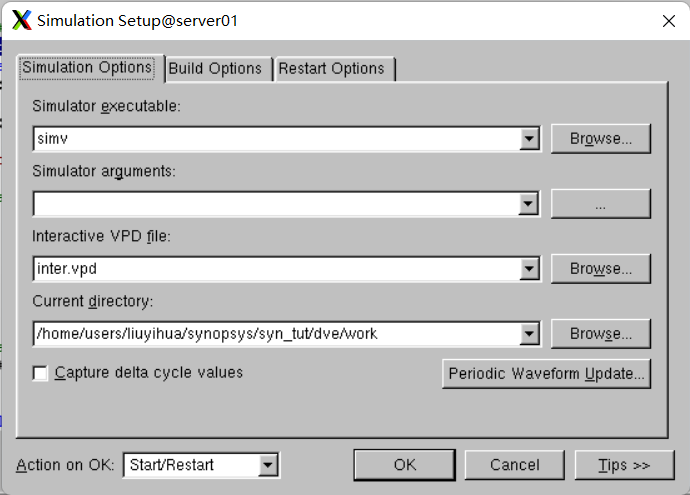
\includegraphics[width=\textwidth]{images/27.png}
        \caption{Simulation setup.}
    \end{figure}
    The Simulation setup has the following options:
    \begin{itemize}
        \item \textit{Simulator Executable} - specifies the name of a simulator executable.
        \item \textit{Simulator arguments} - identifies the simulator arguments.
        \item \textit{Interactive VPD file} - specifies the name of the VPD file. VPD files (design database files) are platform-independent, versioned files into which you can dump the selected signals during simulation. DVE gets hierarchy, value change, and some assertion information from these files.
        \item \textit{Current directory} - specifies the full path of the simulator executable.
    \end{itemize}
    \begin{figure}[H]
        \centering
        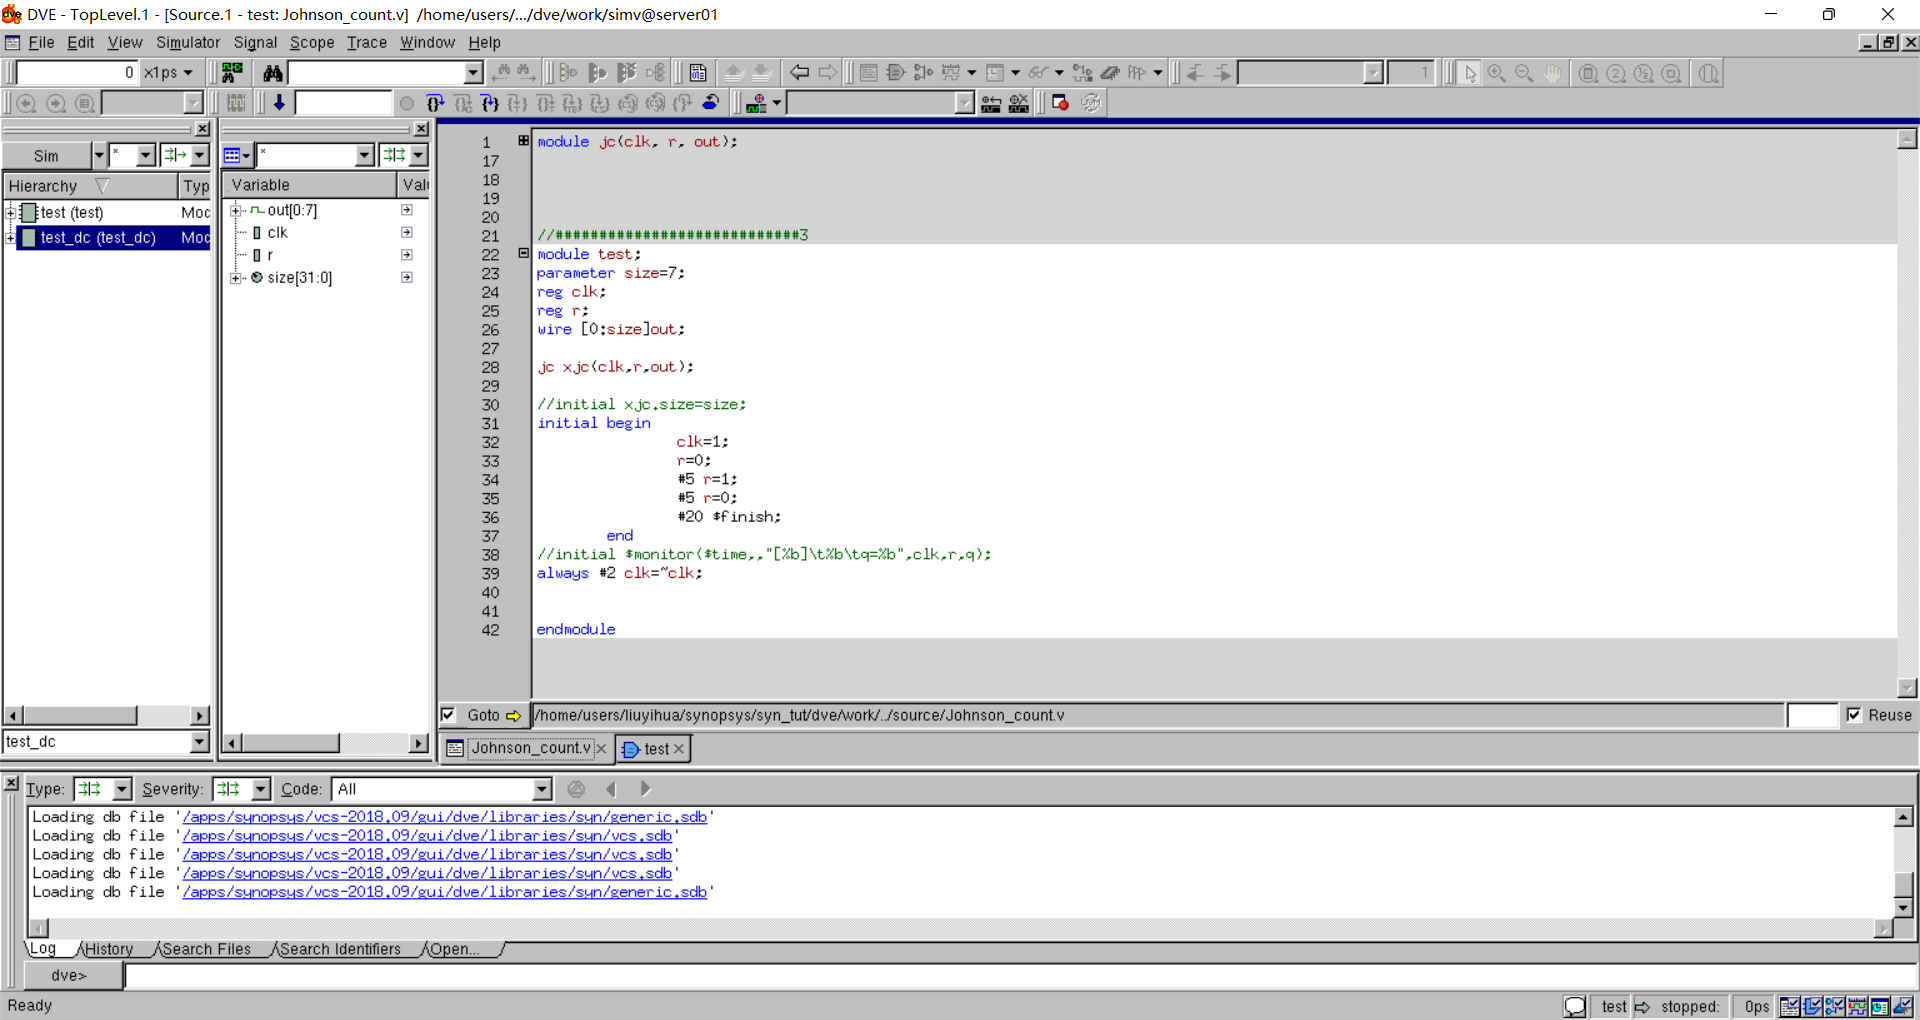
\includegraphics[width=\textwidth]{images/28.png}
        \caption{Overview of DVE window.}
    \end{figure}
    A TopLevel window contains
    \begin{enumerate}
        \item frame,
        \item menus, 
        \item toolbars,
        \item status bar, 
        \item pane targets.
    \end{enumerate}
\end{enumerate}
\subsection{Viewing a Waveform}
\begin{itemize}
    \item \textbf{Hierarchy Pane} - displays the scope hierarchy of the design.
    \item \textbf{Data Pane} - displays the variables of the selected scopes of the Hierarchy pane.
    \item \textbf{Source View} - Displays the source code and supports source code relative features, such as tracing driver or load, and setting line breakpoints.
    \item \textbf{List View} - provides a table view to display the values of signals over time.
    \item \textbf{Schematic View} - provides a module-based schematic to display the connectivity of the object.
    \item \textbf{Assertions View} - displays the summary of assertion results of simulations, including the success, failures, and incomplete ones.
\end{itemize}
To view the simulation waveform for this testbench, select all of the signals in the wave pane (clk, out, r, size), right-click, and select "Add To Waves > New Wave View". You should see an empty wave window after this step.

Using Simulator Menu->Start/Continue (shortcut is the F5 key) or the down arrow button on the toolbar, the simulation until a breakpoint is hit, the simulation finishes, or for the duration specified in the set Continue Time dialog box or toolbar time entries. When the simulation is running, the red circle Stop icon is activated, and you can click to stop the simulation.
\begin{figure}[H]
    \centering
    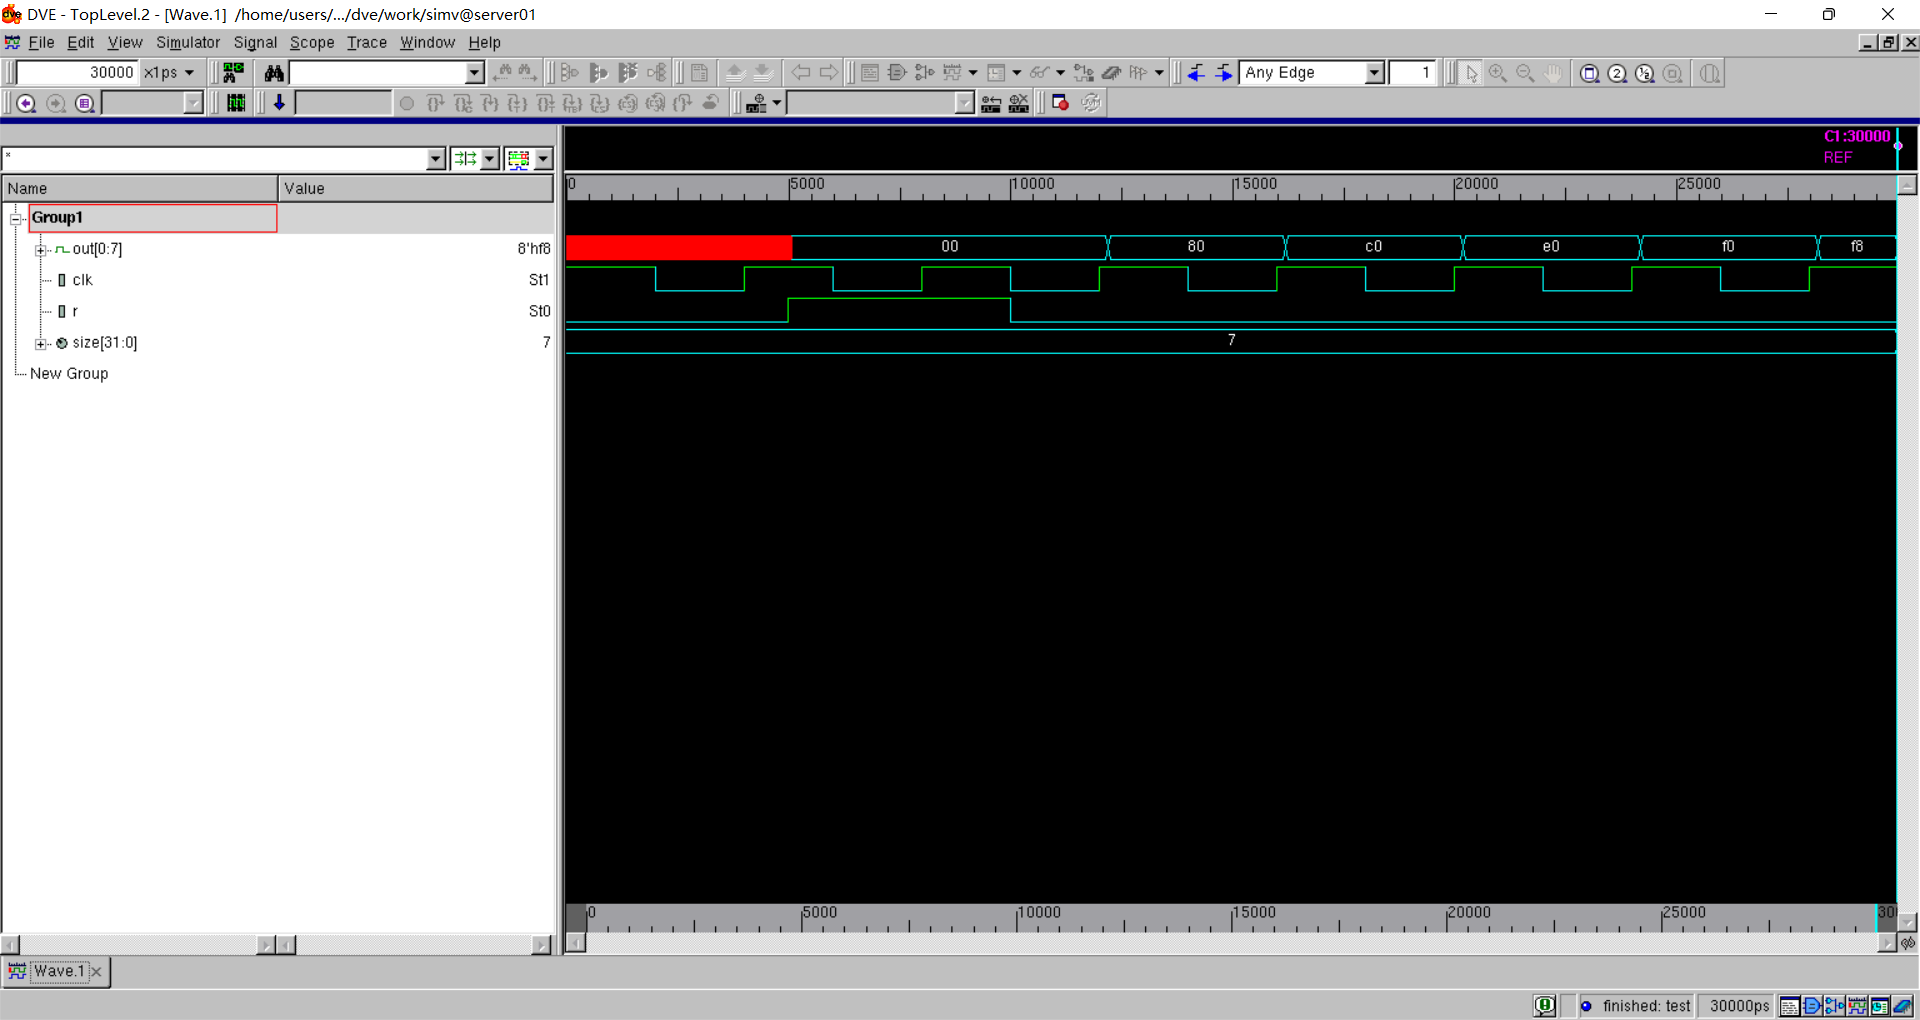
\includegraphics[width=\textwidth]{images/29.png}
    \caption{Wave view window.}
\end{figure}
\textit{Right-click the waveform view and click Zoom->Zoom Full to view the full range of the waveform}.
\subsection{Tracing Drivers and Loads}\label{SDrv}
\begin{enumerate}
    \item Trace drivers and loads of a signal at any time to see the drivers/loads that caused a value change and see all the drivers/loads that possibly contributed to a signal value.
    \item Select a signal in the signal view pane.
    \item Right-click and select Trace Drivers or Trace Loads. When a driver is traced, a new Driver pane will be created if none exists in the current top-level frame. If a driver pane exists, the driver information will be added to the top of the list.
\end{enumerate}
Additionally, the first driver will be highlighted in the Source view and annotated with a blue node in the gutter. In the
Wave view, double-click on a waveform to see its drivers (Figure \ref{f30}).

Link the Driver panes to the Source view in the same top-level frame and Path Schematic view. The link to the radio
buttons at the top right of the pane shows the current linked windows. By linking a Source and Schematic view,
when the object is selected in the Drivers pane, the object will also be selected in the linked views.
\begin{figure}[H]
    \centering
    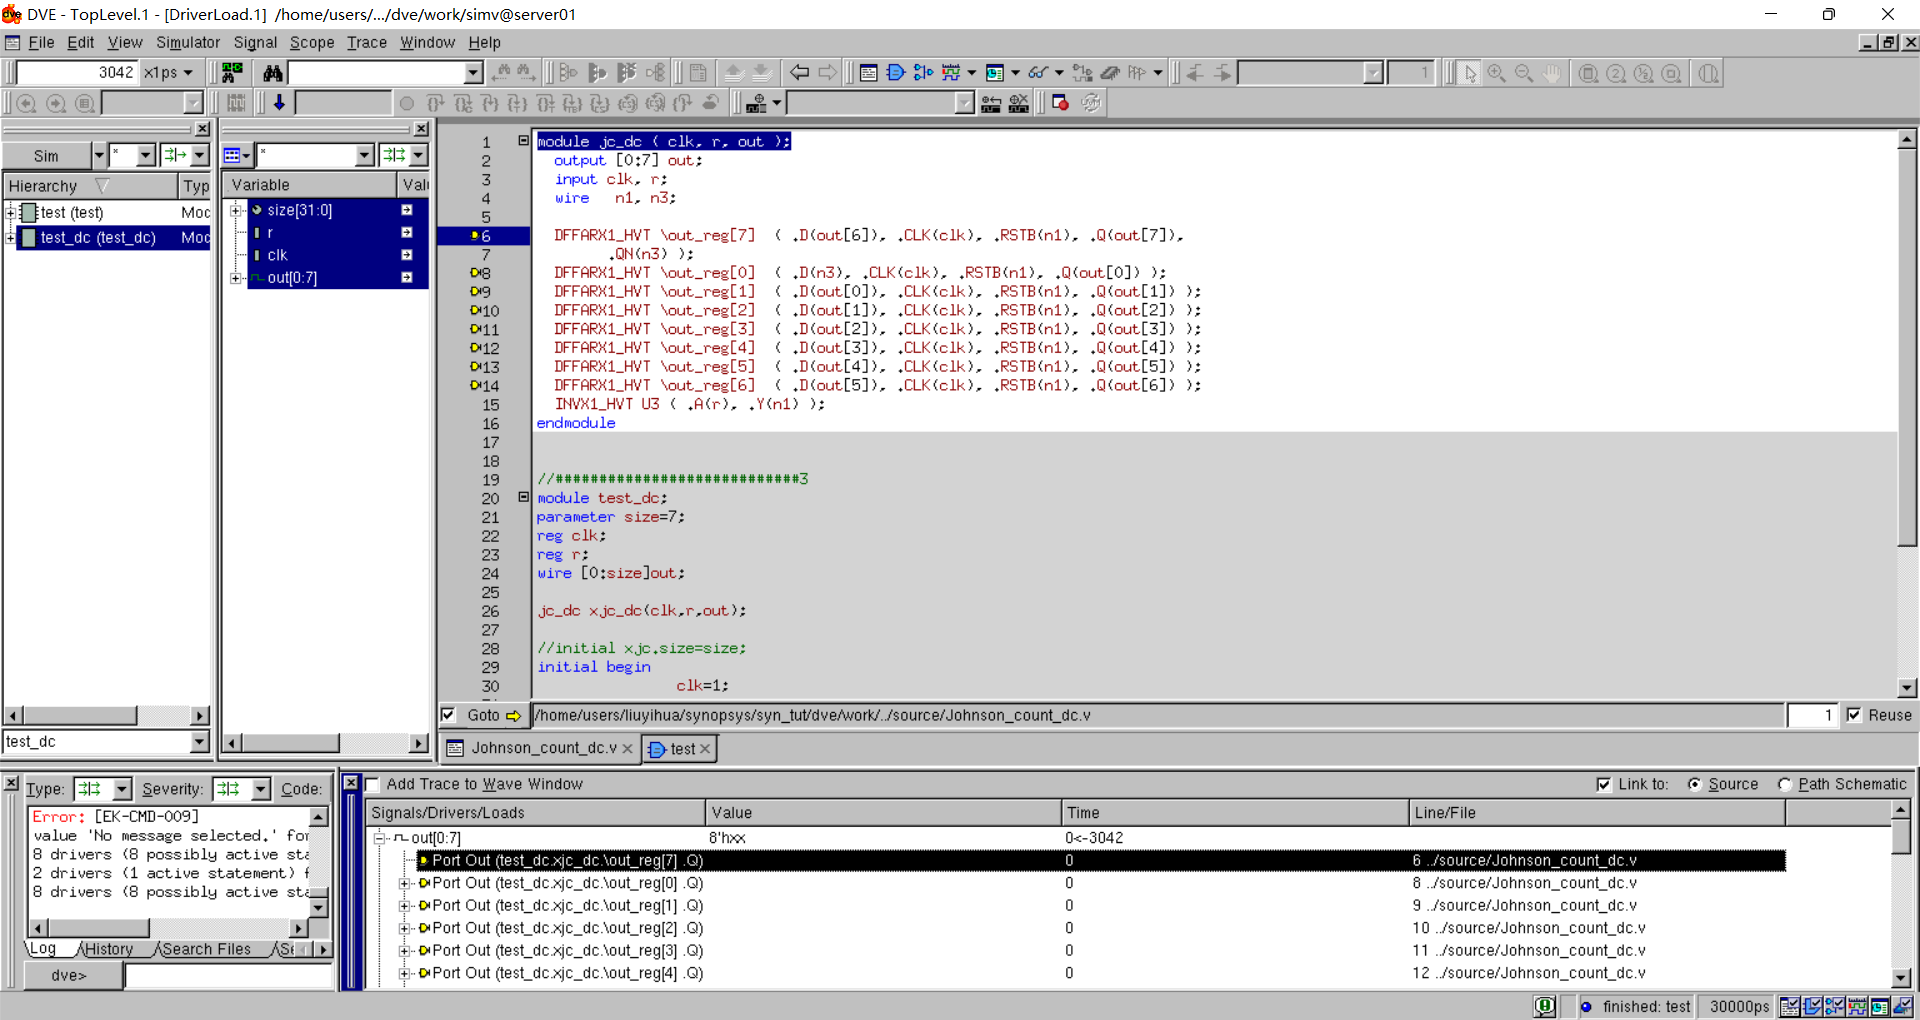
\includegraphics[width=\textwidth]{images/30.png}
    \caption{TopLevel window with tracing drivers and loads.}
    \label{f30}
\end{figure}
\subsection{Comparing Signals, Scopes, and Groups}\label{SComp}
For comparing individual signals with the same bit numbers, scopes (for comparing variable children), buses, or groups of
signals from one or two designs.

To view a comparison
\begin{enumerate}
    \item Select one or two signals, signal groups, scopes, or buses from the Signal pane of the Wave view.
    \item Right-click and select Compare...
    \item Click Load Reference Signals/Scopes and select the text file with the signals and scopes to reference.
    \begin{itemize}
        \item Note 1: If comparing two designs from the root, then the reference waveform region and test waveform region can be empty.
        \item Note 2: If you don't have a reference file, you can skip this step and still compare the signals you have in your design.
    \end{itemize}
    \item Click the More Options button (Figure \ref{f31})\\
    The dialog box is expanded, and additional options are displayed.
    \begin{figure}[H]
        \centering
        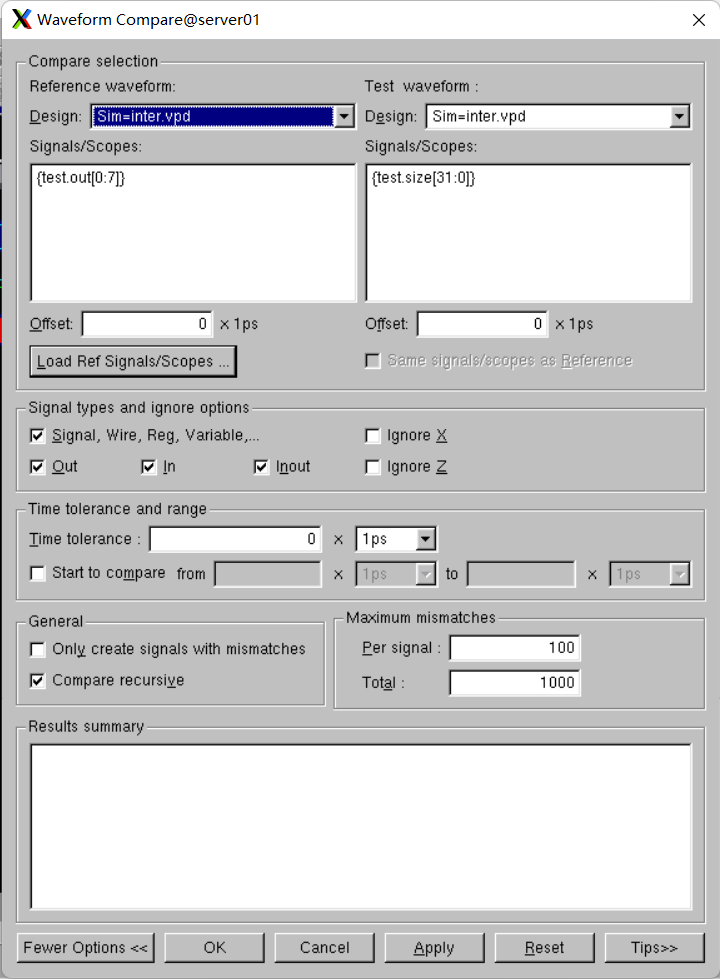
\includegraphics[width=0.8\textwidth]{images/31.png}
        \caption{The Waveform Compare dialog box.}
        \label{f31}
    \end{figure}
    \item In the Signal types and ignore options section, select the signal types to compare and select ignore options.\\
    For example, if Ignore X is selected and if the reference signal value is X, there is always a match, whatever the values of the Test Signal.
    \item Enter a Time Tolerance to filter out mismatch values that have time ranges smaller than the tolerance range.
    \item In the General section, select to compare recursively or to only create signals with mismatches.
    \item Click Apply to start the comparison and keep the dialog box open. Or click OK to start the comparison and close the dialog box (to open it at any time from the Signal pane CSM). Results are displayed in the current Wave view.
    % Show Compare Info seems to be removed in newer versions of DVE
    % \item Select a result in the Wave view, right-click and select Show Compare Info.
\end{enumerate}
\subsection{(Optional) Selecting signal in the Schematic View}\label{SSch}
\textit{You can open the Schematic View by right-clicking the module in the Hierarchy view and clicking "Show Schematic" or clicking the "Show Schematic" button on the toolbar or pressing Ctrl+2}.

To select a signal in the Schematic view
\begin{enumerate}
    \item Enter the signal name in the Find toolbar box in the Schematic view and then click the Find Next toolbar button. The signal is highlighted in the schematic.
    \item With the signal selected, click the Trace Drivers toolbar button or select the Trace Drivers menu item. The signal is highlighted in purple.
\end{enumerate}
\subsection{Using User-defined Radixes}\label{SRadix}
This section describes how to create, edit, import, and export user-defined radices. You can define a custom mnemonic mapping from values to strings for display in the Wave view.

To create, delete, import, and export a user-defined radix
\begin{enumerate}
    \item Select Signal->Set Radix->User-Defined->Edit...
    \item Click New, enter a radix name and then hit the Enter key on your keyboard. All buttons on the Edit User-defined Radix get enabled. \textit{Remember to switch Tcl based to Table based}.
    \item Click Add Row to activate a row for the user-defined radix and perform the following steps:
    \begin{itemize}
        \item Select the text and background colors for each row entry.
        \item Select the radix, click a cell in the Value and Display column, then enter the values. The radix is edited.
    \end{itemize}
    \item Select a row and then click Delete Row. The row is deleted.
    \item Select a radix from the Radix Table Name drop-down and click the Delete button. The radix is deleted.
    \item Click Import, then browse and select the desired radix. The radix is imported.
    \item Click Export, select the radix and then enter a radix name. The radix is exported.
    \item Select the Apply user-defined radix to selected signal(s) checkbox (Figure \ref{f32}). The user-defined radix is applied to the selected signal in the Wave view.
    \item Click OK or Apply to save the user-defined radix.
\end{enumerate}
\begin{figure}[H]
    \centering
    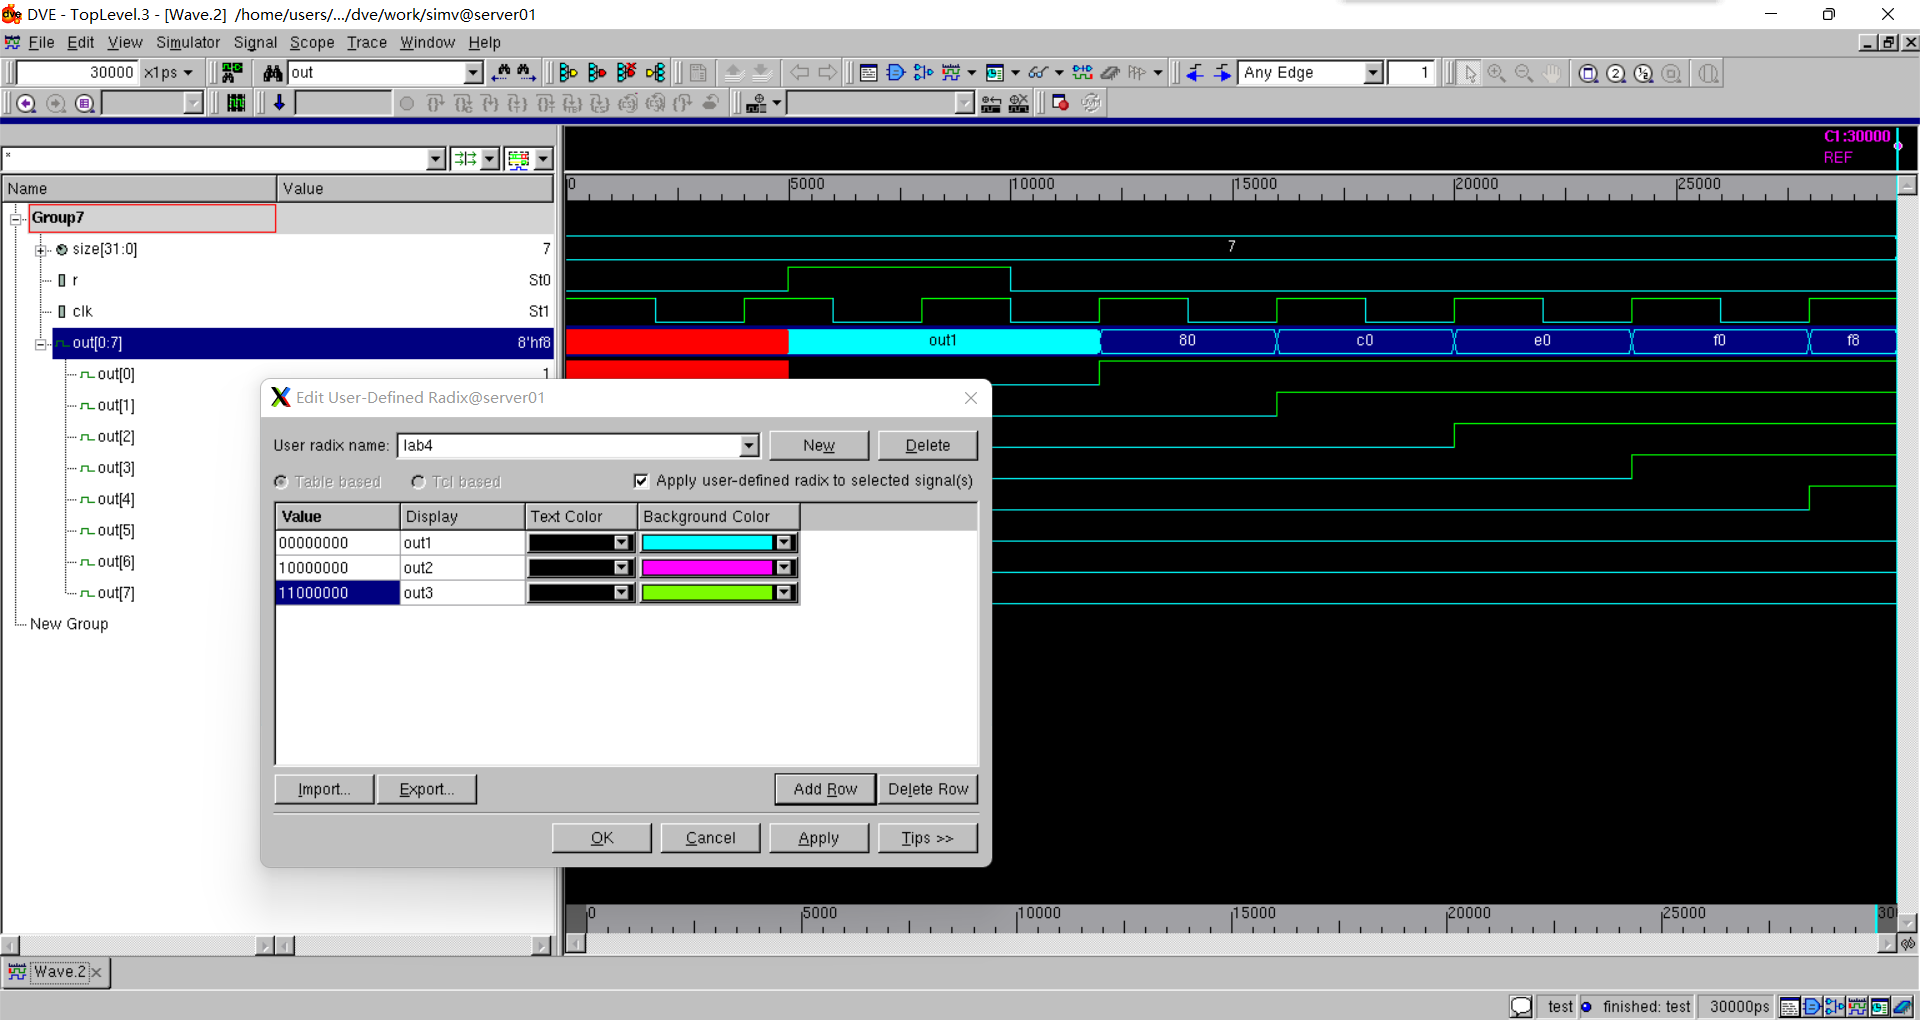
\includegraphics[width=\textwidth]{images/32.png}
    \caption{The Edit User-defined Radix dialog box with Wave view window.}
    \label{f32}
\end{figure}
\textit{Export the User-Defined Radix as a TXT file.}

To exit DVE write exit in the command line on the console.
\begin{minted}{text}
DVE> exit
\end{minted}

\newpage
\section{Logic Synthesis}
Synopsys Design Compiler (DC) is composed of
\begin{itemize}
    \item Design Compiler Graphical
    \item DC Ultra (TM)
    \item DFTMAX (TM)
    \item Power Compiler (TM)
    \item DesignWare (R)
    \item DC Export (TM)
    \item Design Vision (TM)
    \item HDL Compiler (TM)
    \item VHDL Compiler (TM)
    \item DFT Compiler
    \item Design Compiler (R)
\end{itemize}
\subsection{Design Compiler}
\subsubsection{Introduction}
Synopsys provides an integrated RTL synthesis solution. Using Design Compiler tools, you can:
\begin{itemize}
    \item Produce fast, area-efficient ASIC designs by employing user-specified or standard-cell libraries
    \item Translate designs from one technology to another
    \item Explore design tradeoffs involving design constraints such as timing, area, and power under various loading, temperature, and voltage conditions
    \item Synthesize and optimize finite state machines
    \item Integrate netlist inputs and netlist or schematic outputs into third-party environments while still supporting delay information and place and route constraints
    \item Create and partition hierarchical schematics automatically
\end{itemize}

\subsubsection{Basic synthesis flow}
\begin{figure}[H]
    \centering
    \begin{overpic}[scale=1]{images/14.png}
        \put(-41,0){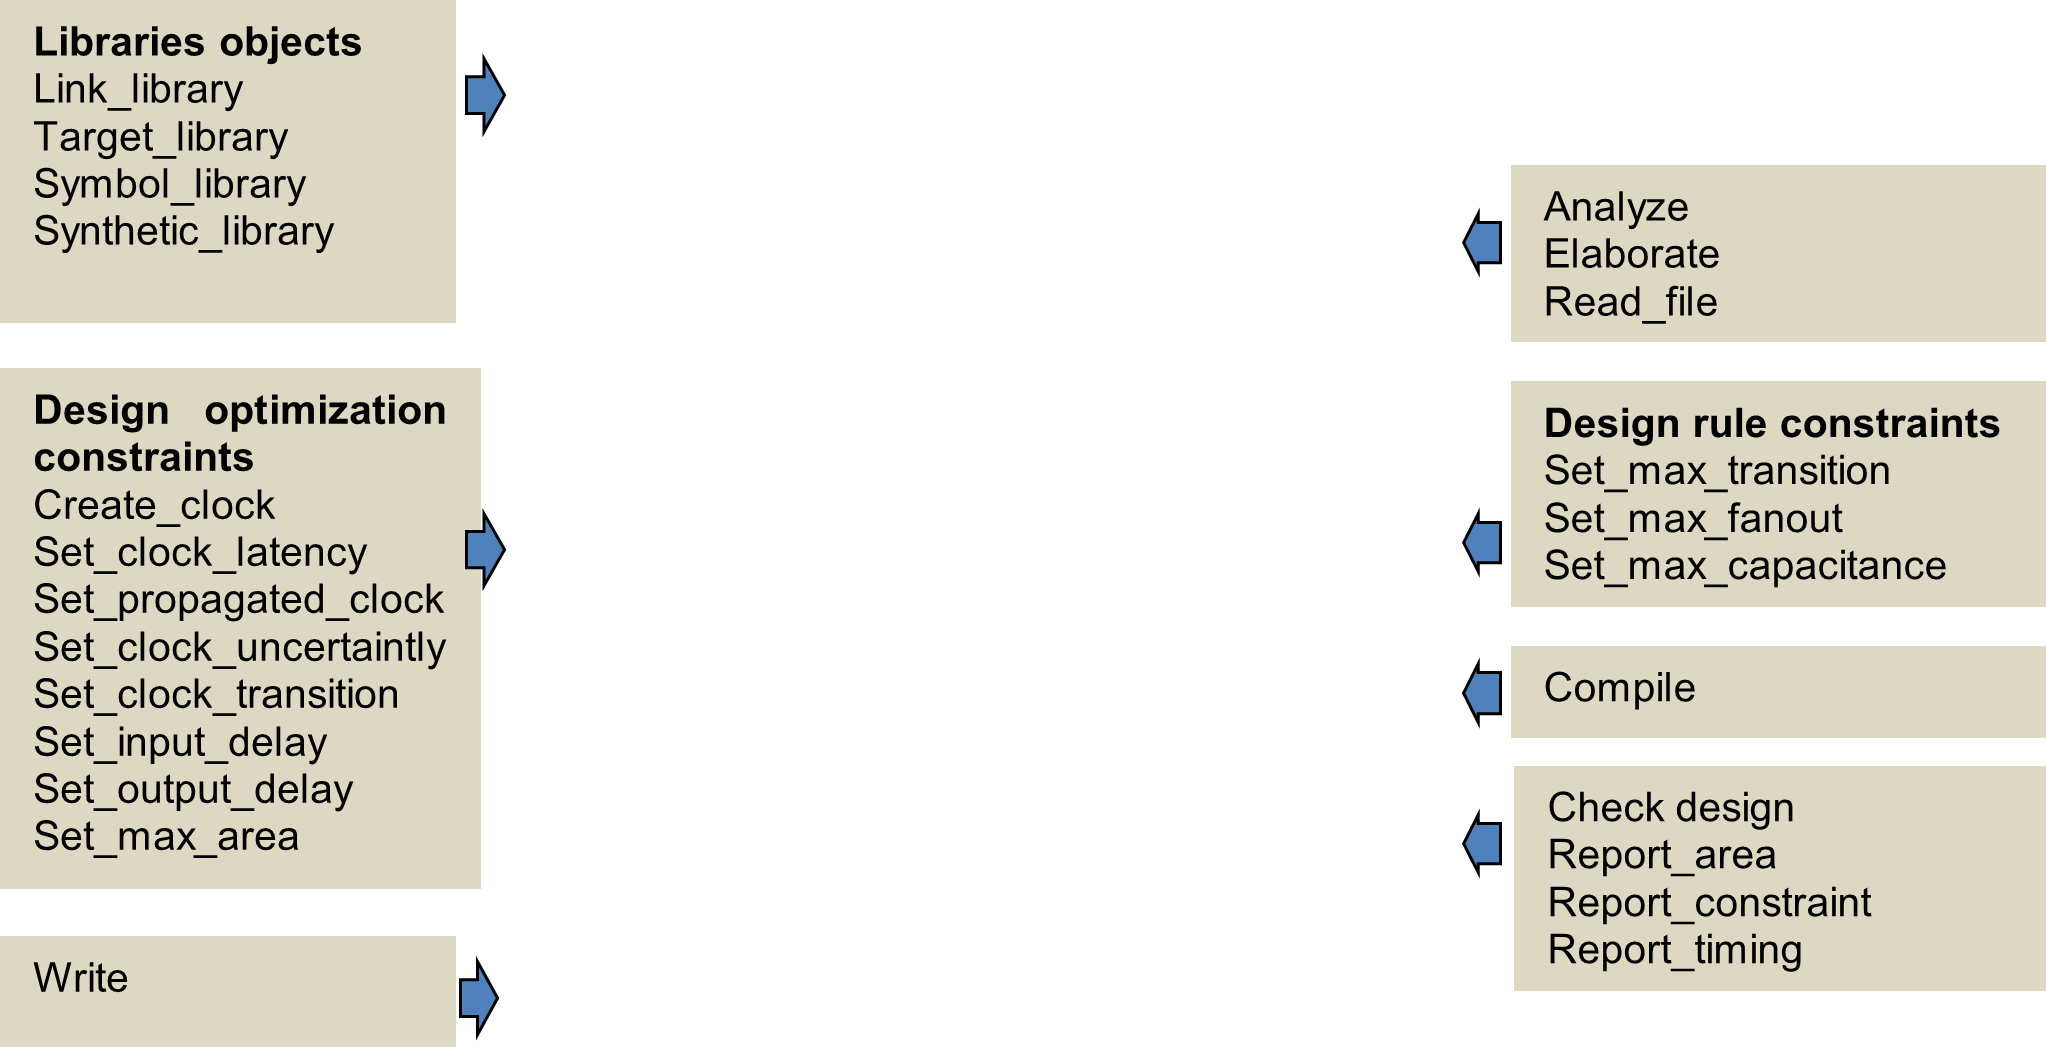
\includegraphics[scale=1]{images/16.png}}  
    \end{overpic}
    \caption{Basic synthesis flow.}
\end{figure}
% \subsection{DC's input and output files}
\begin{figure}[H]
    \centering
    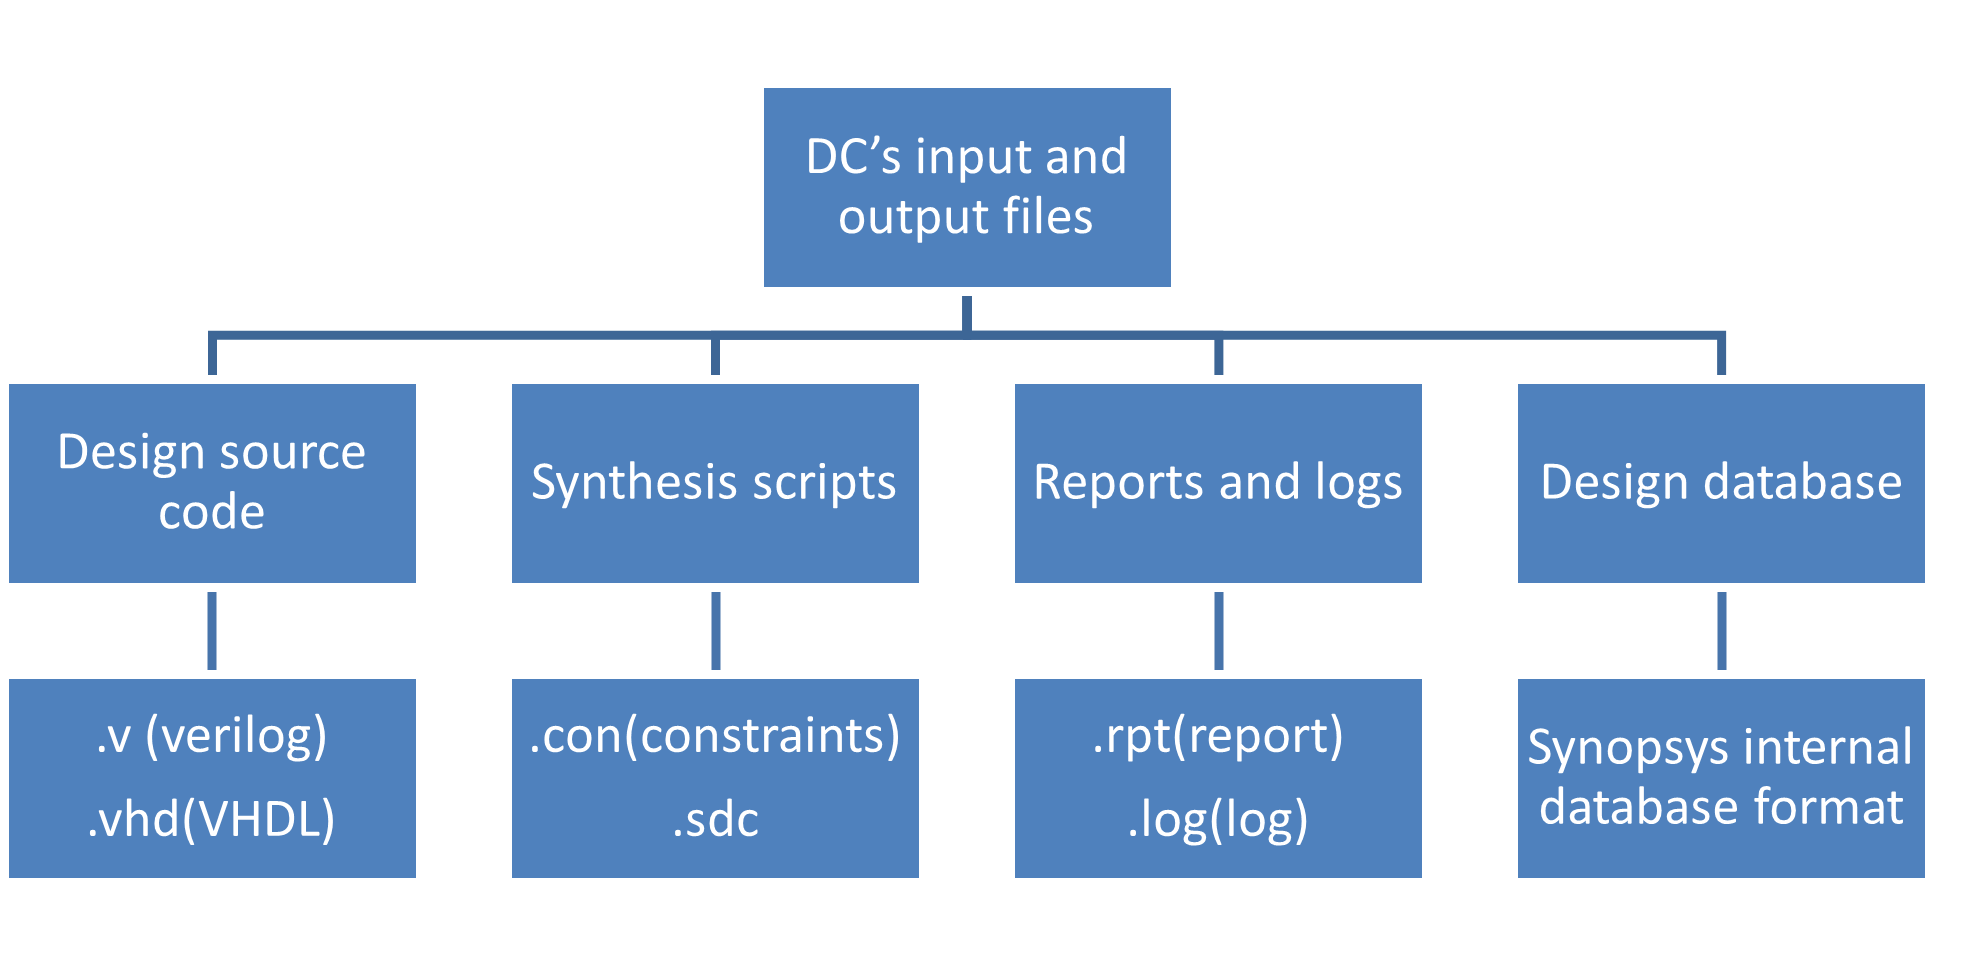
\includegraphics[width=\textwidth]{images/15.png}
    \caption{DC's input and output files.}
\end{figure}
\subsubsection{Tasks}\label{SDCTask}
\begin{enumerate}
    \item First, create a synopsys/syn\_tut directory if one does not already exist. Make sure to unzip the /home/Flow/Synopsys/Scripts/Dc\_32\_paths.zip directory in the syn\_tut directory and move \texttt{dc\_32} out.
    % \begin{enumerate}
    If using Synopsys 90nm EDK, make a directory dc\_90 and copy contents of dc\_32 to it. Start Design Compiler graphical user interface (GUI) from the \texttt{work} directory. To start it, use the following commands:
    \begin{minted}{bash}
cd synopsys
mkdir syn_tut
cd syn_tut
cd dc_32  # or cd dc_90
cd work
dc_shell
    \end{minted}
    Then in the DC Shell, run \texttt{start\_gui}. This opens the DC top-level GUI window:
    \begin{figure}[H]
        \centering
        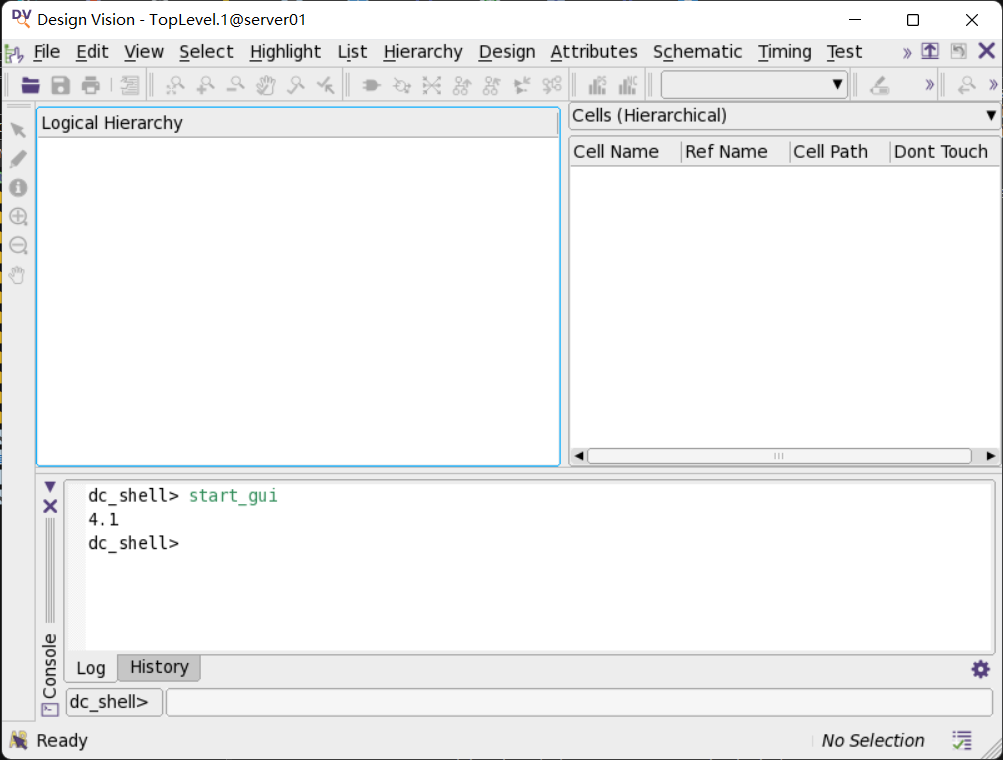
\includegraphics[width=\textwidth]{images/17.png}
        \caption{DC Top-Level GUI Window.}
    \end{figure}
    % \end{enumerate}
    Of course, you can use \texttt{dc\_shell} commands during the flow without GUI, which is even much more convenient as long as you are familiar with them.
    \item Second, setup the libraries:\\
    Go to File -> Setup and then set the Link and Target libraries to
    \begin{itemize}
        \item The \texttt{search\_path} is set to ". /apps/synopsys/syn-2020.09/libraries/syn\\
        /apps/synopsys/syn-2020.09/dw/syn\_ver /apps/synopsys/syn-2020.09/dw/sim\_ver" by default. For Synopsys 90nm EDK, append /home/pdk/synopsys\_edk/edk90/\\
        synopsys\_design\_flow\_using\_90nm\_library/models/ to it (the \texttt{models} directory is the same as the \texttt{dc/models} directory); for Synopsys 32/28nm EDK, append /home/pdk/synopsys\_edk/edk32/models (the \texttt{edk32} directory is the same as the \texttt{/home/Flow/Synopsys/Scripts/icc\_32/ref} directory).
        \item For Synopsys 90nm EDK, write "* saed90nm\_typ\_ht.db" in \texttt{link\_path}; for Synopsys 32/28nm EDK, write "* saed32hvt\_tt1p05v25c.db".
        \item For Synopsys 90nm EDK, write "saed90nm\_typ\_ht.db" in \texttt{target\_library}; for Synopsys 32/28nm EDK, write "saed32hvt\_tt1p05v25c.db".
        \item You can leave the \texttt{symbol\_library} as it is (\texttt{your\_library.sdb}). When you add the libraries, also make sure you explicitly remove the "your\_library.db" default; otherwise, you will get a warning message later.
        \begin{figure}[H]
            \centering
            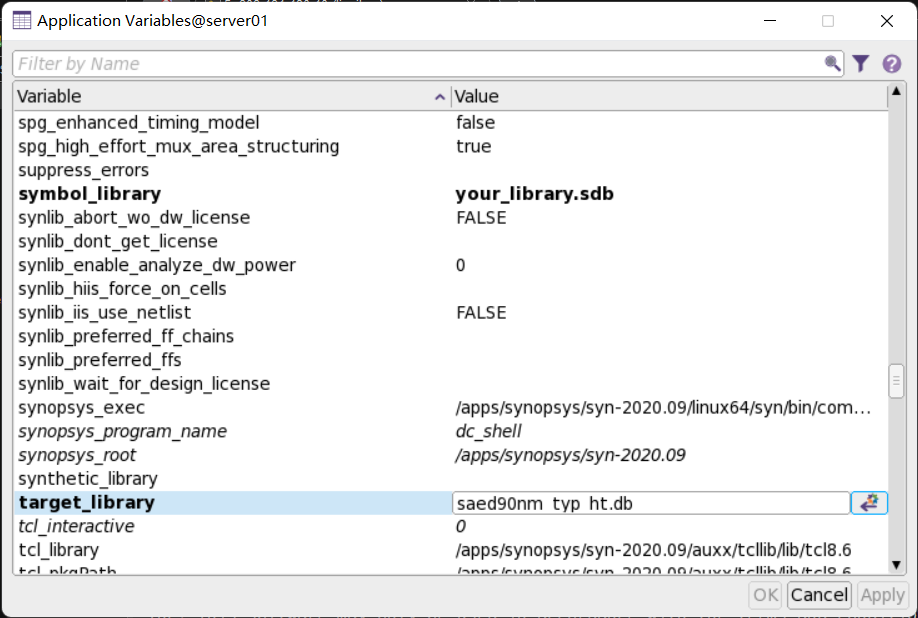
\includegraphics[width=\textwidth]{images/18.png}
            \caption{Application Variables Window.}
        \end{figure}
    \end{itemize}
    \begin{minted}[breaklines,breakanywhere]{tcl}
set_app_var search_path {. /apps/synopsys/syn-2020.09/libraries/syn /apps/synopsys/syn-2020.09/dw/syn_ver /apps/synopsys/syn-2020.09/dw/sim_ver /home/pdk/synopsys_edk/edk90/synopsys_design_flow_using_90nm_library/models}
set_app_var target_library saed90nm_typ_ht.db
set_app_var link_path  {* saed90nm_typ_ht.db}
    \end{minted}
    \begin{minted}[breaklines,breakanywhere]{tcl}
set_app_var search_path {. /apps/synopsys/syn-2020.09/libraries/syn /apps/synopsys/syn-2020.09/dw/syn_ver /apps/synopsys/syn-2020.09/dw/sim_ver /home/pdk/synopsys_edk/edk32/models}
set_app_var target_library saed32hvt_tt1p05v25c.db
set_app_var link_path  {* saed32hvt_tt1p05v25c.db}
    \end{minted}
    The asterisk means all the libraries in the memory.
    \item Third, read in the source file. Read design commands are derived from the read\_file -format VHDL or read\_file -format Verilog commands. In our design, we used -format Verilog:
    \begin{figure}[H]
        \centering
        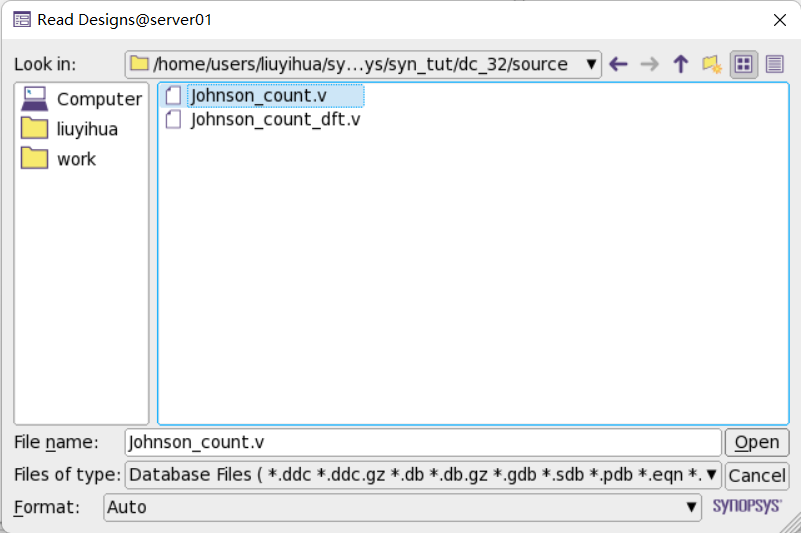
\includegraphics[width=\textwidth]{images/19.png}
        \caption{Read Designs Box.}
        \label{f19}
    \end{figure}
    Go to File -> Read and set Johnson\_count.v as the source file as seen in Figure \ref{f19}:
    \begin{minted}[breaklines,breakanywhere]{tcl}
read_file -format verilog {/home/users/<username>/synopsys/syn_tut/dc_32/source/Johnson_count.v}
    \end{minted}
    \item Fourth, use the \texttt{analyze} and \texttt{elaborate} commands.\\
    To run the analyze command: Go to File -> Analyze. After Analyze is clicked, the window seen in Figure \ref{f20} should appear. The analyze command does the following:
    \begin{itemize}
        \item Reads an HDL source file
        \item Checks it for errors (without building generic logic for the design)
        \item Creates HDL library objects in an HDL-independent intermediate format
        \item Stores the intermediate files in a defined location
    \end{itemize}
    \textit{Click the small button on the right of the textbox of "File names in analysis order". In the pop-up dialog "Specify File names in analysis order:@server01", click the "+ Add" button, click the small button on the right of the textbox, and select ../source/Johnson\_count.v. Click OK. The File names in analysis order are now ../source/Johnson\_count.v. Click OK.}
    \begin{figure}[H]
        \centering
        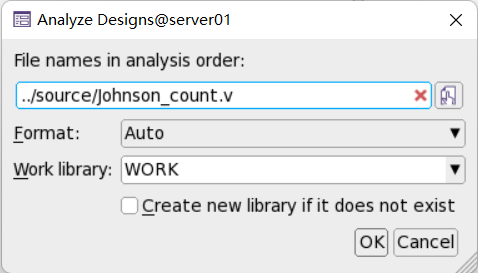
\includegraphics[width=0.6\textwidth]{images/20.png}
        \caption{Analyze Designs Box.}
        \label{f20}
    \end{figure}
    If the analyze command reports errors, fix them in the HDL source file and run \texttt{analyze} again. After a design is analyzed, reanalyze it only when it changes.
    \begin{minted}[breaklines,breakanywhere]{tcl}
analyze -library WORK -format verilog {../source/Johnson_count.v}
    \end{minted}
    \textit{The expected output is}:
    \begin{minted}[breaklines]{text}
Running PRESTO HDLC
Compiling source file ../source/Johnson_count.v
Presto compilation completed successfully.
    \end{minted}
    \textit{Click the Save button to save the design to johnson\_count.ddc}
    \begin{minted}[breaklines,breakanywhere]{tcl}
write -hierarchy -format ddc
    \end{minted}
    To run the \texttt{elaborate} command: Go to File -> Elaborate. After Elaborate is clicked, the window seen in Figure \ref{f21} should appear. The \texttt{elaborate} command does the following:
    \begin{itemize}
        \item Translates the design into a technology-independent design (GTECH) from the intermediate files produced during the analysis
        \item Allows changing of parameter values defined in the source code
        \item Allows VHDL architecture selection
        \item Replaces the HDL arithmetic operators in the code with DesignWare components
        \item Automatically executes the link command, which resolves design references
    \end{itemize}
    \textit{In the Elaborate Designs@server01 dialog, enter "DEFAULT" to the Library textbox, then johnson\_count(verilog) is automatically selected as the Design. Click OK}
    \begin{figure}[H]
        \centering
        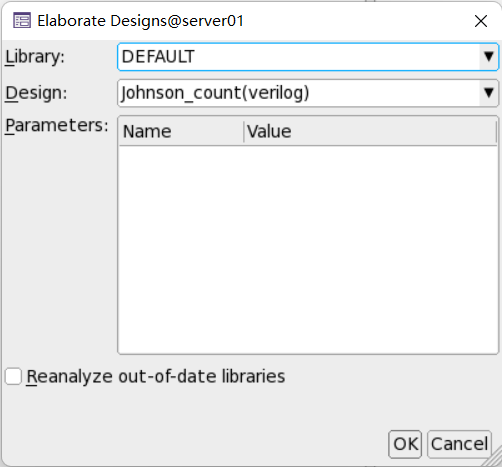
\includegraphics[width=0.6\textwidth]{images/21.png}
        \caption{Elaborate Designs Box.}
        \label{f21}
    \end{figure}
    \begin{minted}[breaklines,breakanywhere]{tcl}
elaborate Johnson_count -architecture verilog -library DEFAULT
    \end{minted}
    \textit{The expected output is}:
    \begin{minted}{text}
    Running PRESTO HDLC

Inferred memory devices in process
        in routine Johnson_count line 8 in file
                '../source/Johnson_count.v'.
===============================================================================
|    Register Name    |   Type    | Width | Bus | MB | AR | AS | SR | SS | ST |
===============================================================================
|       out_reg       | Flip-flop |   8   |  Y  | N  | Y  | N  | N  | N  | N  |
===============================================================================
Presto compilation completed successfully. (Johnson_count)
Warning: Design 'Johnson_count' was renamed to 'Johnson_count_1' to avoid
        a conflict with another design that has the same name but
different parameters. (LINK-17)
Elaborated 1 design.
Current design is now 'Johnson_count_1'.
    \end{minted}
    \textit{You can switch between designs from the Design List drop-down list on the toolbar}.
    \item Fifth, for a design to be complete, it needs to be connected to all of the library components and designs it references. So to perform a name-based resolution of design references for the current design, use the \texttt{link} command.
    \begin{minted}[breaklines,breakanywhere]{text}
dc_shell> link
  Linking design 'Johnson_count_1'
  Using the following designs and libraries:
  --------------------------------------------------------------------------
  * (2 designs)               /home/users/<username>/synopsys/syn_tut/dc_32/work/Johnson_count_1.db, etc
  * (2 designs)               /home/users/<username>/synopsys/syn_tut/dc_90/work/Johnson_count_1.db, etc
  saed32hvt_tt1p05v25c (library) /home/pdk/synopsys_edk/edk32/models/saed32hvt_tt1p05v25c.db
  saed90nm_typ_ht (library)   /home/pdk/synopsys_edk/edk90/synopsys_design_flow_using_90nm_library/models/saed90nm_typ_ht.db

1
    \end{minted}
    \item Sixth, The \texttt{check\_design} command needs to be run. The \texttt{check\_design} command checks the internal representation of the current Synopsys Design Constraints for consistency and issues errors and warning messages as appropriate.
    \item Seventh, set design optimization constraints, source the file constr.sdc. The optimization constraints comprise:
    \begin{itemize}
        \item Timing constraints (performance and speed)
        \item Input and output delays (synchronous paths)
        \item Minimum and maximum delay (asynchronous paths)
        \item Maximum area (number of gates)
    \end{itemize}
    Synopsys Design Constraints (SDC) include many commands to indicate designers' constraints. It is a set of commands. In addition to resources in this lab, please refer to the documents for details:
    \begin{itemize}
        \item \url{http://www.vlsi-expert.com/2011/02/synopsys-design-constraints-sdc-basics.html}
        \item \url{http://www.cs.utah.edu/~elb/cadbook/color-figs/Chapter13-Example.pdf}
        \item \url{https://free-online-ebooks.appspot.com/enc/14.17/fetxtcmdref/}
    \end{itemize}
    Using SDC, we can set timing constraints. We want to design a circuit, but we want it to be able to communicate with its neighbor circuits efficiently. Therefore we kind of required to have (for design purposes) outputs loads (as if there is another circuit attached) and input buffer/inverter cell (that drives the input). Since we use cells for the input, we don't need to define the input loads. Those cells already have output loads (cells' outputs are our inputs). We use registers for inputs other than the clock. In this case, we used d-flip-flop.\\
    Synopsys 32/28nm Generic Library contains predefined cell/gates/blocks. You can use \texttt{gedit} to open the lib file \texttt{models/saed90nm\_typ\_ht\_pg.lib}. This library is for high threshold voltage (HVT) cells. NBUFFX16\_HVT is a buffer for clock signals. A is its input, and Y is its output. A is going to be used by ScanMasterClock. SDFFARX1\_HVT is a Scan Pos Edge DFF (D flip-flop) w/Async Low-Active Reset. D is its input, and Q is its output. You can see that we assign these pins with our signal. These cells drive our input signals, so their output will be our input. Normal inputs need to come to our circuit in an order with the help of the clock; also, they need to be kept in short-term memory. Register cells are for this.\\
    To source constraints with .sdc (Synopsys Design Constraints) format:
    \begin{minted}[breaklines,breakanywhere]{text}
dc_shell> source ../source/constr.sdc
    \end{minted}
    \item After all steps mentioned above are completed, right-click on the Johnson\_count\_1 located under the Logical Hierarchy tab. Then select Schematic View, \textit{double-click the Johnson\_count\_1 cell to expand the hierarchy, switch the "Cells (Hierarchical)" view to the "Pins/Ports" view}, and a Schematic seen in Figure \ref{f22} should appear.
    \begin{figure}[H]
        \centering
        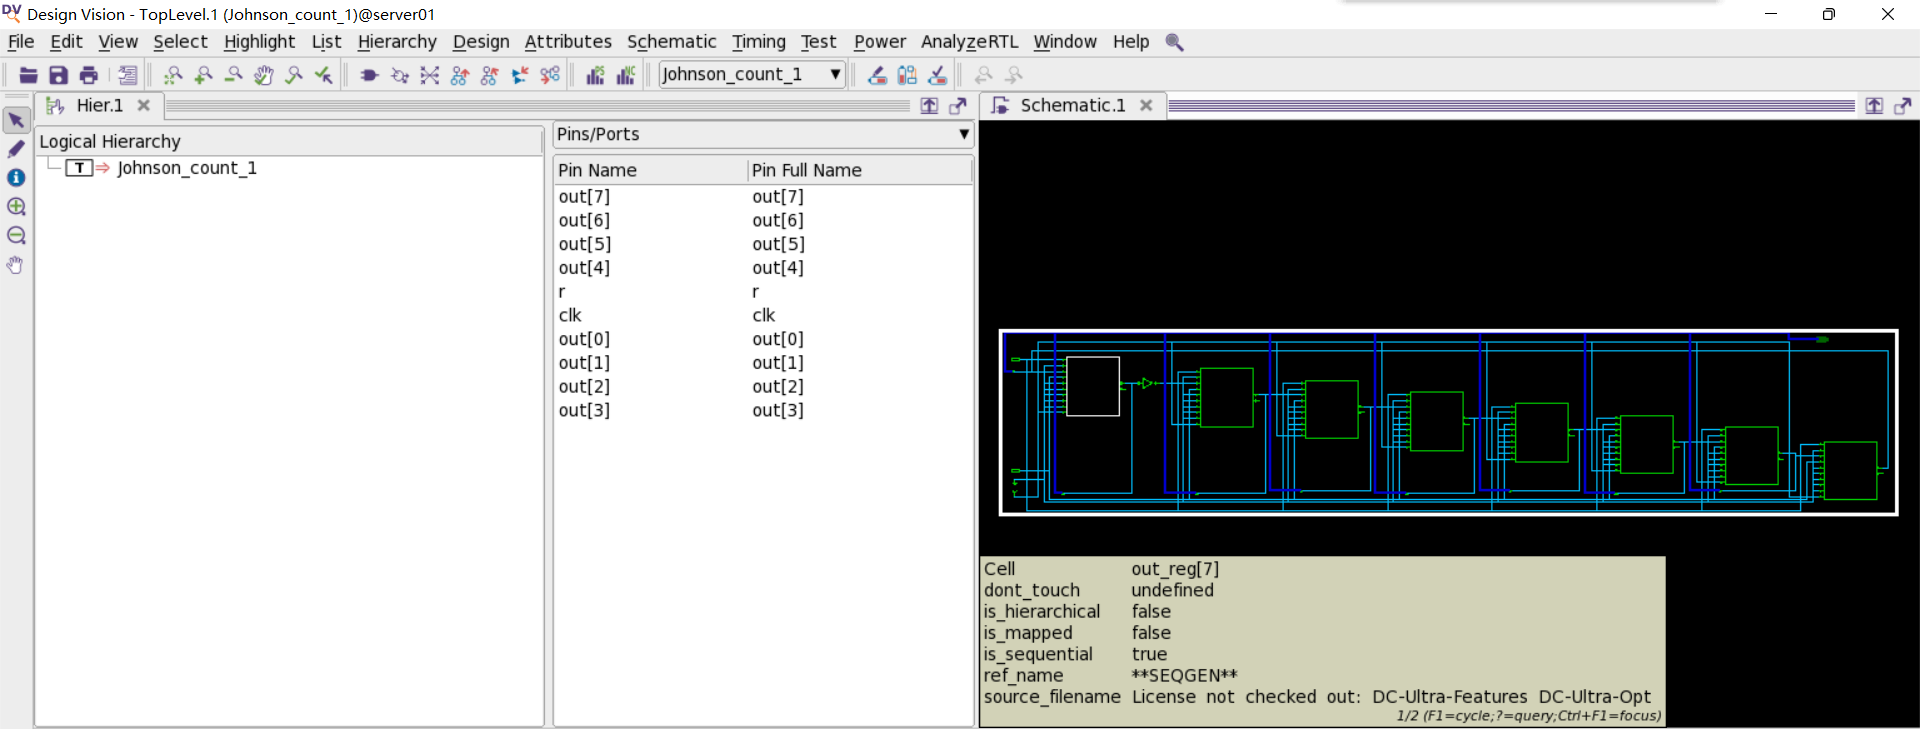
\includegraphics[width=\textwidth]{images/22.png}
        \caption{Design View From DC.}
        \label{f22}
    \end{figure}
    \item The \texttt{compile} command performs logic and gate-level synthesis and optimization on the current design. This command specifies that the sequential elements in the final design must exactly match the descriptions specified in the HDL. The command uses attributes/directives with the -exact\_map option to ensure that the results of compile are predictable. Optimization is controlled by user-specified constraints on the design. To perform this command use the following:
    \begin{minted}[breaklines,breakanywhere]{text}
dc_shell> compile -exact_map
    \end{minted}
    The compiled design produces a gate-level description seen in Figure \ref{f23}. To retrieve this image, once again right-click on the Johnson\_count\_1 located under the Logical Hierarchy tab, \textit{expand the hierarchy}, then select Schematic View.
    \begin{figure}[H]
        \centering
        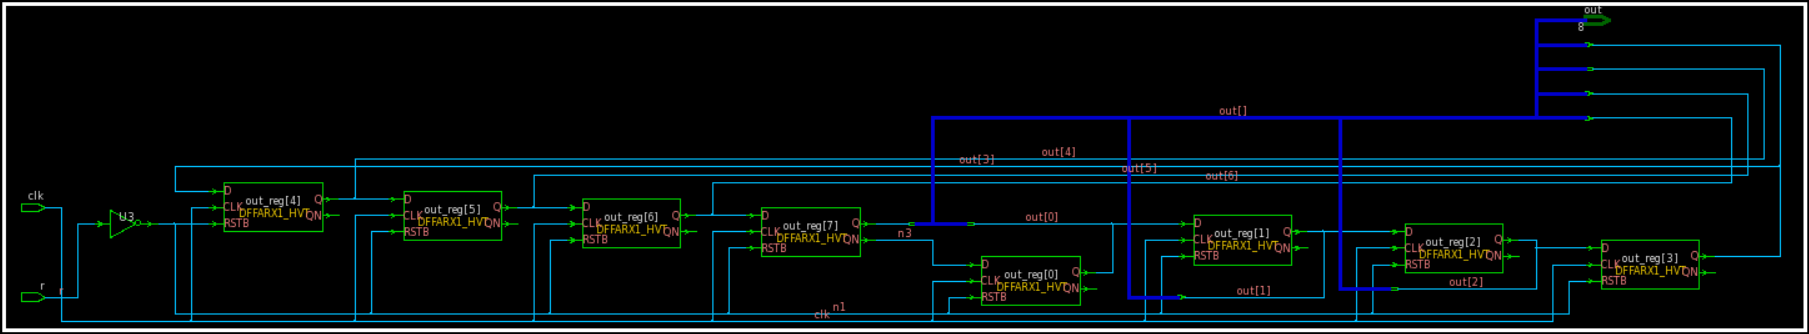
\includegraphics[width=\textwidth]{images/23.png}
        \caption{Design View From DC After Compile.}
        \label{f23}
    \end{figure}
    \item Design Compiler can generate numerous reports on the results of design synthesis and optimization. Reports are used to analyze and resolve any design problems or to improve synthesis results.\\
    In \texttt{dc\_shell}, run \texttt{report\_area}, \texttt{report\_constraint}, and \texttt{report\_timing}.
    \item Write a design from memory to .ddc (Synopsys internal database format) by using the command below (format is still .v and .vhdl):
    \begin{minted}[breaklines,breakanywhere]{text}
dc_shell> write -hierarchy -format verilog -output ../results/Johnson_count_dcl.v
    \end{minted}
    \textit{At any time, for permission issues like "Error: Can't open export file" ... (EXPT-4) "Error: Write command failed. (UID-25)", you can write to another path}.
    \item The next step will be to run DFT Compiler. In order to start DFT Compiler (Design for Test Compiler), reset the design using the following command:
    \begin{minted}[breaklines,breakanywhere]{text}
dc_shell> reset_design
    \end{minted}
\end{enumerate}
\subsection{DFTC (Design for Test Compiler)}
\subsubsection{Introduction}
DFT Compiler is used to:
\begin{itemize}
    \item check RTL and mapped designs for DFT violations
    \item insert scan chains into designs
    \item export all the required files for downstream tools
\end{itemize}
DFT Compiler requires the user to specify a scan style in order to perform scan synthesis. A scan style dictates the appropriate scan cells to insert during optimization. The scan style, which is selected is used on all modules of design. There are three types of scan styles available in DFT Compiler:
\begin{itemize}
    \item Multiplexed flip-flop
    \item Clocked scan
    \item Level-sensitive scan design
\end{itemize}
To specify the scan style of this design, the following command is used:
\begin{minted}[breaklines,breakanywhere]{text}
dc_shell> set test_default_scan_style
\end{minted}
Using this command sets the scan style to the default multiplexed\_flip\_flop scan style.
\subsubsection{Basic Scan Synthesis Flow}
\begin{figure}[H]
    \centering
    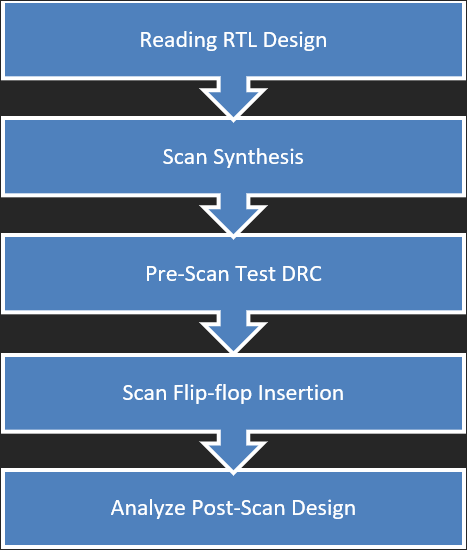
\includegraphics[width=0.6\textwidth]{images/24.png}
    \caption{Basic Scan Synthesis Flow.}
\end{figure}
\subsubsection{Tasks}\label{SDFTCTask}
\begin{enumerate}
    \item First, specify the scan style. To specify the scan style of this design, use the command introduced above.
    \item Second, read the design by using the following command:
    \begin{minted}[breaklines,breakanywhere]{text}
dc_shell> read_verilog ../source/Johnson_count_dft.v
    \end{minted}
    After reading the design, see the schematic view of Johnson\_count by clicking \texttt{johnson\_count} in the Logical Hierarchy and click Menu->Schematic->New Schematic View. \textit{Still, expand the hierarchy. You can right-click the schematic view and click "Zoom Fit All" to have a better view}.
    \begin{figure}[H]
        \centering
        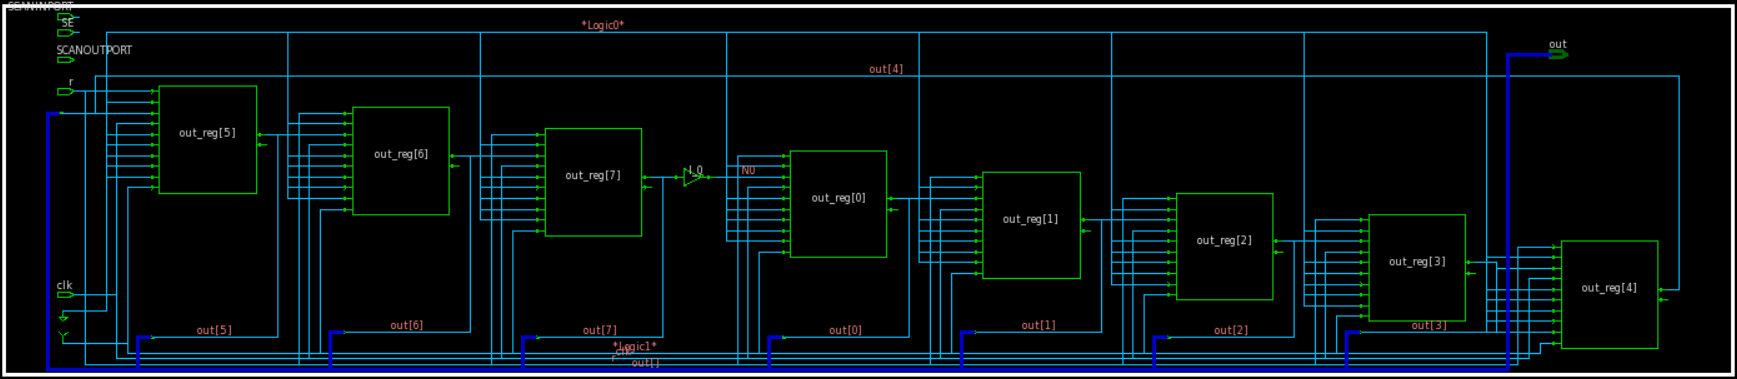
\includegraphics[width=\textwidth]{images/25.png}
        \caption{Schematic view of Johnson\_count before DFT.}
        \label{f25}
    \end{figure}
    The intended schematic view is shown in Figure \ref{f25}.
    \item Third, source constraints with .sdc format by using the command below:
    \begin{minted}[breaklines,breakanywhere]{text}
dc_shell> source ../source/constr.sdc
    \end{minted}
    \item Fourth, assign the port types to the signals that will be used in DFT. For example, ScanMasterClock, Reset, and ScanEnable. To give port types to signals, use the following commands:
    \begin{minted}[breaklines,breakanywhere]{tcl}
set_dft_signal -view exist -type ScanMasterClock -timing {45 55} -port clk
set_dft_signal -view exist -type Reset -active 1 -port r
set_dft_signal -view exist -type ScanEnable -active 1 -port SE
report_dft_signal -view exist
    \end{minted}
    \begin{itemize}
        \item set\_dft\_signal specifies the DFT signal types for DRC and DFT insertion.
        \item -view exist option shows that ports which already exist in design, and if the port must use first time, apply the \texttt{-view spec} option.
        \item -active option specifies the active sense of the port (high or low).
    \end{itemize}
    \item Sixth, create a test protocol to configure the design for scan test by using the command:
    \begin{minted}[breaklines,breakanywhere]{text}
dc_shell> create_test_protocol
    \end{minted}
    This creates a test protocol that DFT Compiler uses for test design rule checking as well as pattern generation and vector formatting steps.
    \item Seventh, check the design respective to the multiplexed-flip-flop scan style, which is defined using set test\_default\_scan\_style. Run design rule checking by using the following command:
    \begin{minted}[breaklines,breakanywhere]{text}
dc_shell> dft_drc
    \end{minted}
    This command checks violations. If violations are reported, change the RTL code and repeat steps 5 and 6. If no violations are reported, proceed to scan synthesis.
    \begin{figure}[H]
        \centering
        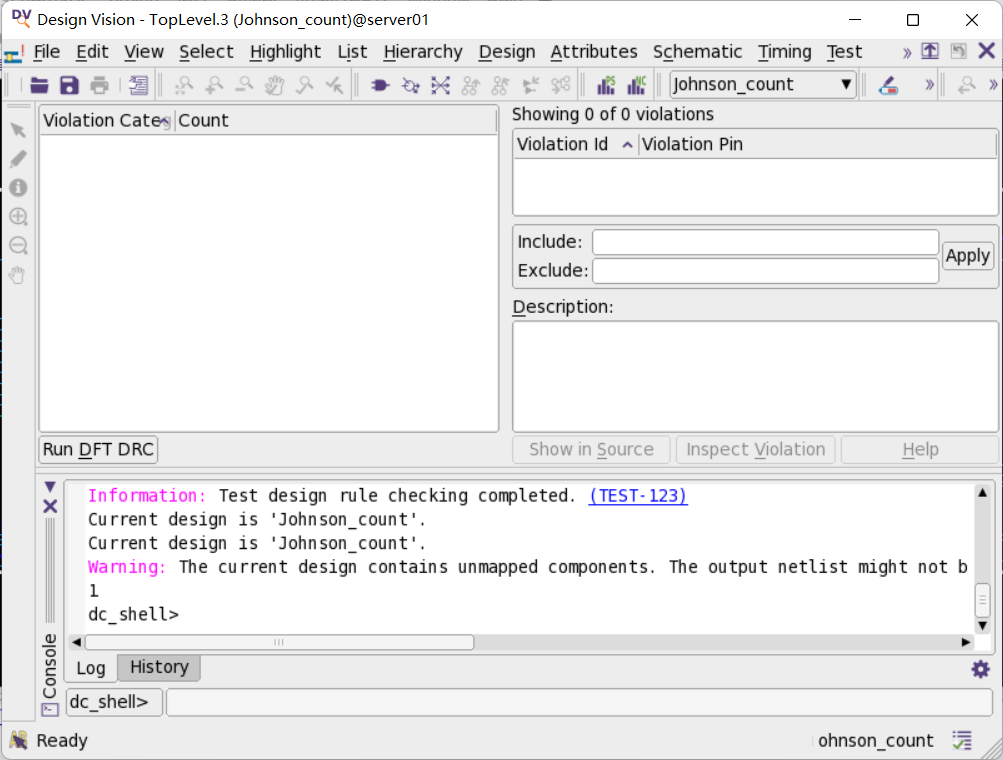
\includegraphics[width=\textwidth]{images/26.png}
    \end{figure}
    If there are no violations after dft\_drc, it means that the protocol is working, so write out the complete protocol with .spf format for later use in the Mapped Flow.
    \begin{minted}[breaklines,breakanywhere]{text}
dc_shell> write_test_protocol -out ../source/Johnson_count_test.spf
    \end{minted}
    \item Eighth, create a clock object and define its waveform in the current design. 1000 specifies the period of the clock waveform in library time units. Then set input delays on SCANINPORT and on SE relative to a clock signal.
    \begin{minted}[breaklines,breakanywhere]{tcl}
create_clock clk -period 1000
set_input_delay 250 SCANINPORT -clock clk
set_input_delay 150 SE -clock clk
    \end{minted}
    \item Scan Insertion will change the design to escape from negative effects (such as Scan Registers' possible influence that may increase the area of the schematic and increase the fan-out on the nets), which must be taken into consideration during the synthesis. That's why synthesis uses scan triggers to prevent schematic feature changes. To realize this, use the following command:
    \begin{minted}[breaklines,breakanywhere]{text}
dc_shell> compile -scan -ungroup_all
    \end{minted}
    \item For a design to be complete, it needs to be connected to all of the library components and designs it references. So to perform a name-based resolution of design references for the current design, use the link command. The references must be located and linked to the current design in order for the design to be functional. The purpose of this command is to locate all of the designs and library components referenced in the current design and connect (link) them to the current design.
    \begin{minted}[breaklines,breakanywhere]{text}
dc_shell> link
    \end{minted}
    \item To read a test protocol file into memory.
    \begin{minted}[breaklines,breakanywhere]{text}
dc_shell> read_test_protocol ../source/Johnson_count_test.spf
    \end{minted}
    \textit{The output is}:
    \begin{minted}[breaklines,breakanywhere]{text}
Warning: a protocol already exists in mode 'all_dft' and will be deleted. (TEST-1401)
... deleting protocol from the mode 'all_dft' ...

... Reading /home/users/<username>/synopsys/syn_tut/dc_90/source/Johnson_count_test.spf ...
... STIL version 1.0 ( Design 2005 CTL P2001.10) ...
... SignalGroups  ...
... Timing  ...
... Procedures all_dft_protocol: "multiclock_capture" "allclock_capture" "allclock_launch" "allclock_launch_capture" ...
... MacroDefs all_dft_protocol: "test_setup" ...
Warning: Reading in a test protocol after specifying signals will cause the signals to be cleared from the protocol and the model.  (TEST-1714)
Read protocol for mode all_dft
1
    \end{minted}
    \item Use -view spec in order to define the scan structure.
    \begin{minted}[breaklines,breakanywhere]{tcl}
set_dft_signal -view spec -port SCANINPORT -type ScanDataIn
set_dft_signal -view spec -port SCANOUTPORT -type ScanDataOut
set_dft_signal -view exist -port SE -type ScanEnable
    \end{minted}
    \item Set the DFT insertion configuration for the current design.
    \begin{minted}[breaklines,breakanywhere]{text}
dc_shell> set_dft_insertion_configuration -preserve_design_name true
    \end{minted}
    \texttt{-preserve\_design\_name true} specifies whether to preserve the design name when writing from the tool to the database during DFT insertion. Valid values are true to preserve the design name and false to permit renaming the design. The default value is false.
    \item To specify the scan chain design.
    \begin{minted}[breaklines,breakanywhere]{text}
dc_shell> set_scan_configuration -chain_count 1
    \end{minted}
    \texttt{-chain\_count 1} specifies a positive integer for the number of chains that insert\_dft is to build. If not specified, insert\_dft builds the minimum number of scan chains consistent with clock mixing constraints.
    \item Before performing scan insertion, you can preview the scan design by specifying the \texttt{preview\_dft} command. This command generates a scan chain that satisfies the scan specifications on your current design and displays the scan chain design. Previews, but does not implement, the test points, scan chains, and on-chip clocking control logic to be added to the current design.
    \begin{minted}[breaklines,breakanywhere]{text}
dc_shell> preview_dft
    \end{minted}
    \item After previewing the design, it is ready to assemble the scan chains by using \texttt{insert\_dft} command. It adds scan circuitry (either internal scan or boundary-scan) to the current design.
    \begin{minted}[breaklines,breakanywhere]{text}
dc_shell> insert_dft
    \end{minted}
    \item Set the \texttt{fix\_multiple\_port\_nets} attribute to a specified value on the current design. To buffer logic constants, use the \texttt{-buffer\_constants} option with the \texttt{-all} option. \texttt{-buffer\_constants} option buffers logic constants instead of duplicating them.
    \begin{minted}{tcl}
set_fix_multiple_port_nets -all -buffer_constants
compile -scan -incremental
    \end{minted}
    \item Run design rule checking again and display area information for the current design.
    \begin{minted}{tcl}
dft_drc -coverage_estimate
report_area
    \end{minted}
    \texttt{-coverage\_estimate} generates test coverage estimate at the end of design rule checking.
    \item Write a design from memory to a file with format .sdc (Synopsys internal database format), also format .v and .vhdl.
    \begin{minted}[breaklines,breakanywhere]{text}
dc_shell> write -format verilog -h -o ../results/Johnson_count_dc.v
    \end{minted}
    \item Write a design with Standard Delay Format (SDF).
    \begin{minted}[breaklines,breakanywhere]{text}
dc_shell> write_sdf ../results/Johnson_count_dc.sdf
    \end{minted}
    \item To exit DFT Compiler write exit in the command line.
    \begin{minted}[breaklines,breakanywhere]{text}
dc_shell> exit
    \end{minted}
\end{enumerate}

\newpage
\section{Getting Started with OpenLane and SkyWater PDK}
\subsection{Introduction}
\href{https://theopenroadproject.org/}{The OpenROAD Project} is founded by the University of California, San Diego VLSI CAD Laboratory, cooperated with the University of Michigan, ARM, University of Minnesota, Arizona State University, etc. The main product of the OpenROAD project is the \href{https://github.com/The-OpenROAD-Project/OpenROAD}{OpenROAD} App. OpenROAD is a foundational building block in open-source digital flows like \href{https://github.com/The-OpenROAD-Project/OpenROAD-flow-scripts}{OpenROAD-flow-scripts}, \href{https://github.com/The-OpenROAD-Project/OpenLane}{OpenLane} from \href{https://efabless.com/}{Efabless}, Silicon Compiler Systems, as well as \href{https://github.com/idea-fasoc/OpenFASOC}{OpenFASoC} for mixed-signal design flows. The OpenROAD project supports two main flow controllers:
\begin{itemize}
    \item \href{https://github.com/The-OpenROAD-Project/OpenROAD-flow-scripts}{OpenROAD-flow-scripts} - Supported by the OpenROAD project
    \item \href{https://github.com/The-OpenROAD-Project/OpenLane}{OpenLane} - Supported by \href{https://efabless.com/}{Efabless}
\end{itemize}
In this lab, we will mainly focus on OpenLane.
\begin{figure}[H]
    \centering
    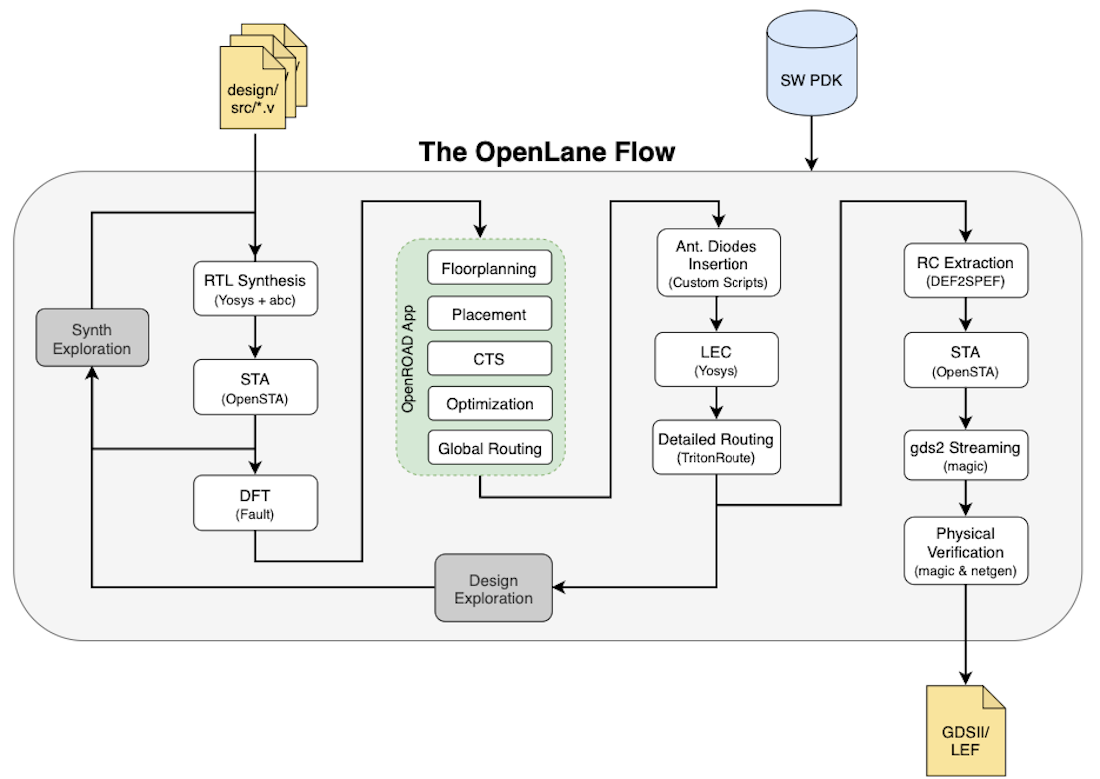
\includegraphics[width=\textwidth]{images/33.png}
    \caption{OpenLane Architecture.}
    \label{f33}
\end{figure}
OpenLane is an automated RTL to GDSII flow based on several components, including OpenROAD, Yosys, Magic, Netgen, CVC, SPEF-Extractor, KLayout, and a number of custom scripts for design exploration and optimization. The flow performs all ASIC implementation steps from RTL all the way down to GDSII.

The SkyWater Open Source PDK is a collaboration between Google and \href{https://www.skywatertechnology.com/}{SkyWater Technology Foundry} to provide a fully open-source Process Design Kit and related resources, which can be used to create manufacturable designs at SkyWater’s facility.

There are a few introductory presentations made by various key contributors to help you understand the project \cite{cs250lab1}:
\begin{itemize}
    \item \href{https://www.youtube.com/watch?v=EczW2IWdnOM}{[FOSSi Dial-Up] Tim Ansell - Skywater PDK: Fully open source manufacturable PDK for a 130nm process}
    \item \href{https://www.youtube.com/watch?v=Vhyv0eq_mLU}{[FOSSi Dial-Up] Mohamed Shalan - OpenLane, A Digital ASIC Flow for SkyWater 130nm Open PDK}
    \item \href{https://www.youtube.com/watch?v=HvWveK2fZt0}{[FOSSi Dial-Up] Mohamed Kassem - The striVe RISC-V SoC Family on SkyWater 130nm}
    \item \href{https://www.youtube.com/watch?v=Svus4uQ_CAA}{[FOSSi Dial-Up] James Stine - Designing new 130nm cells for SkyWater 130nm}
\end{itemize}
The repository provides five sky130 standard cell libraries:
\begin{itemize}
    \item \href{https://github.com/The-OpenROAD-Project/openlane/blob/master/regression_results/benchmark_results/SW_HD.csv}{sky130\_fd\_sc\_hd}
    \item \href{https://github.com/The-OpenROAD-Project/openlane/blob/master/regression_results/benchmark_results/SW_HS.csv}{sky130\_fd\_sc\_hs}
    \item \href{https://github.com/The-OpenROAD-Project/openlane/blob/master/regression_results/benchmark_results/SW_MS.csv}{sky130\_fd\_sc\_ms}
    \item \href{https://github.com/The-OpenROAD-Project/openlane/blob/master/regression_results/benchmark_results/SW_LS.csv}{sky130\_fd\_sc\_ls}
    \item \href{https://github.com/The-OpenROAD-Project/openlane/blob/master/regression_results/benchmark_results/SW_HDLL.csv}{sky130\_fd\_sc\_hdll}
\end{itemize}

\subsection{Setting up the OpenLane flow}
Please follow the official documentation \url{https://openlane.readthedocs.io/en/latest/getting_started/installation.html}. For Windows users, deploying OpenLane on WSL2 is recommended: \url{https://docs.docker.com/desktop/windows/wsl/} \url{https://learn.microsoft.com/en-us/windows/wsl/tutorials/wsl-containers} because Windows can dynamically allocate memory for WSL. Some operations need a huge amount of memory, so you can automatically make full use of your memory during the process without many trials and errors. If using virtual machines, please allocate enough memory (at least 4 GiB) for your virtual machines. If you failed to \texttt{make} or start docker "docker: Cannot connect to the Docker daemon at unix:///var/run/docker.sock. Is the docker daemon running?.", please start Docker Desktop for Windows first. If there are errors stopping \texttt{make}
\begin{minted}[breaklines]{text}
requests.exceptions.ConnectionError: ('Connection aborted.', RemoteDisconnected('Remote end closed connection without response'))
\end{minted}
Please read the Troubleshooting \ref{ATVolare}. After \texttt{make}, the sky130A and sky130B PDKs are prepared under the \texttt{pdks/volare} directory. Since OpenLane and SkyWater SKY130 PDK are under active development and the latter one is still an experimental preview or alpha release, there may be versioning issues. Even worse, the developers of OpenLane and SkyWater SKY130 PDK have very bad habits of using Git - they push all commits to the master/main branch every time without previously testing them rather than separate several branches or at least maintain a "develop" branch. Even worse, they instruct users to always start from the master/main branch rather than a tag or a release. The version of OpenLane that is tested by the TA is the commit 32da932761213af689f10088d671e1e3dc38f273 (tag: 2022.10.13). The Sky130 PDK version is de752ec0ba4da0ecb1fbcd309eeec4993d88f5bc. The OpenLane Docker image is tag 32da932761213af689f10088d671e1e3dc38f273-amd64 and the corresponding digest is sha256:92390c610a2204df6551b6cf3f9226e59f30ab17966b0677cd756cda74cb8de6. Unfortunately, during testing, the TA found problems with this version and created pull requests, so this part was cut; just use the latest version. During \texttt{make test}, please note that if you have already set up X11 for WSL 2, it will show:
\begin{minted}[breaklines]{text}
cd /mnt/d/Resources/OpenLane && \
        docker run --rm -v /mnt/d/Resources/OpenLane:/openlane -v /mnt/d/Resources/OpenLane/designs:/openlane/install -v /mnt/d/Resources/OpenLane/pdks:/mnt/d/Resources/OpenLane/pdks -e PDK_ROOT=/mnt/d/Resources/OpenLane/pdks -e PDK=sky130A  --user 1000:1000 -e DISPLAY=:0 -v /tmp/.X11-unix:/tmp/.X11-unix -v /home/<username>/.Xauthority:/.Xauthority --network host efabless/openlane:32da932761213af689f10088d671e1e3dc38f273-amd64 sh -c "./flow.tcl -design spm -tag openlane_test -overwrite"
\end{minted}
After that, if you run \texttt{klayout}, it can open the KLayout window. If not, please set up X11 for WSL 2 first \cite{wslgui}.
\subsection{Adding your designs}\label{SAdd}
Follow \href{https://openlane.readthedocs.io/en/latest/usage/designs.html}{Adding your designs} to create a new design \texttt{lab4} and copy files in \texttt{lab4\_starter} under \texttt{lab4/src}. You are allowed the modify the source code if needed, as long as it is different from the existing designs in the \texttt{design} directory of OpenLane. Using a Tcl configuration file is recommended rather than using a JSON configuration file because the TA has found bugs related to JSON configuration files. You may need to prepare an SDC file under the \texttt{src} directory and configure it in \texttt{config.tcl} or \texttt{config.json}.

Once the run is complete, you should see a new directory in \verb|${OPENLANE_ROOT}/designs/|\\
\texttt{lab4/runs/}. It’ll be named after the UTC time pertaining to the run. Call that subdirectory LATEST\_RUN and descend into it. You should see logs, reports, results, tmp. If you see errors.log or errors.txt, that is bad.
\subsection{(Optional) Regression \& Exploration}\label{SOptReg}
Follow \href{https://openlane.readthedocs.io/en/latest/usage/exploration_script.html}{Regression \& Exploration}. Define a “regression” configuration file in \verb|${OPENLANE_ROOT}/|\\
\texttt{designs/lab4/regression.config} like:
\begin{minted}{text}
CLOCK_PERIOD=(1 2 5 10)
GLB_RT_ADJUSTMENT=(0 0.15)
FP_CORE_UTIL=(10 25 50)
PL_TARGET_DENSITY=(0.05 0.1 0.2)
SYNTH_STRATEGY=(1 3 14)

extra="
"
\end{minted}
There is some documentation for these parameters: \url{https://github.com/efabless/openlane/blob/master/configuration/README.md} now move to \url{https://openlane.readthedocs.io/en/latest/reference/configuration.html}. Set up the regression config and run the regression tool to find the tightest clock timing for the design.
\subsection{(Optional) Tasks}\label{SOptTask}
\begin{enumerate}
    \item Please modify the SDC file and create a case where setup time did not pass, then use the critical as an example and describe how you can fix the timing for that path. Please upload the full timing path and also your answers for fixing the timing violation.
    \item Please modify the SDC file and find the maximum frequency that passes the timing check after routing. Please upload the screenshot of the layout after place and route, and report area and power.
\end{enumerate}

\newpage
\section{Deliverables}
Please add comments or explanations to all the deliverables.
\begin{enumerate}
    \item Section \ref{SVCSTask}: the output of the \texttt{vcs} command.
    \item Section \ref{SDrv}: the screenshot of the TopLevel window with tracing drivers and loads.
    \item Section \ref{SComp}: the screenshot of the Compared Signal Groups in the Wave View.
    \item Section \ref{SSch} (Optional): the screenshot of the Highlighted Signal Groups in the Wave View.
    \item Section \ref{SRadix}: the exported user-defined radix TXT file and the screenshot of the Edit User-defined Radix dialog box with Wave view window.
    \item Section \ref{SDCTask}: the three reports of the area, constraints, and timing in Step 10 and \texttt{Johnson\_count\_dcl.v} in Step 11.
    \item Section \ref{SDFTCTask}: the Preview\_dft report in Step 14, the output of the \texttt{compile} command in Step 16, the area report in Step 17, \texttt{Johnson\_count\_dc.v} in Step 18, and \texttt{Johnson\_count\_dc.sdf} in Step 19.
    \item Section \ref{SAdd}: the screenshot of the output of the run.
    \item Section \ref{SOptReg} (Optional): the \texttt{regression.config} file and the log file and CSV files in the \texttt{regression\_results} directory.
    \item Section \ref{SOptTask} (Optional): the SDC file, the screenshot of the full timing path, the answers for Task 1; the SDC file, the screenshot of the layout after place and route, and the area and power reports for Task 2.
\end{enumerate}

\section{Grading policy}
\begin{table}[H]
    \centering
    \begin{tabular}{|c|c|}
        \hline
        Factors & Percentage \\
        \hline
        Section 4 & 35\% + 2\% bonus \\
        \hline
        Section 5 & 35\% \\
        \hline
        Section 6 & 30\% + 18\% bonus \\
        \hline
    \end{tabular}
\end{table}

\newpage
\appendix
\section{Peer Evaluation Form}
\begin{table}[H]
    \centering
    \begin{tabular}{|c|c|c|c|c|}
        \hline
        Part & Your work & Your partner's work & Your score & Your partner's score \\
        \hline
        Section 4 & & & & \\
        \hline
        Section 5 & & & & \\
        \hline
        Section 6 & & & & \\
        \hline
    \end{tabular}
\end{table}

\newpage
\section{Troubleshooting}\label{A1}
\subsection{VcXsrv XLaunch not working}\label{AXLaunch}
First, make sure there are no other X servers running. Then, please read the reference article \cite{xlaunchcsdn}.
\subsection{Other X server problems}
Please read the reference article \cite{cs252x11}.
\subsection{MobaXterm X server}\label{AMobaX}
\begin{figure}[H]
    \centering
    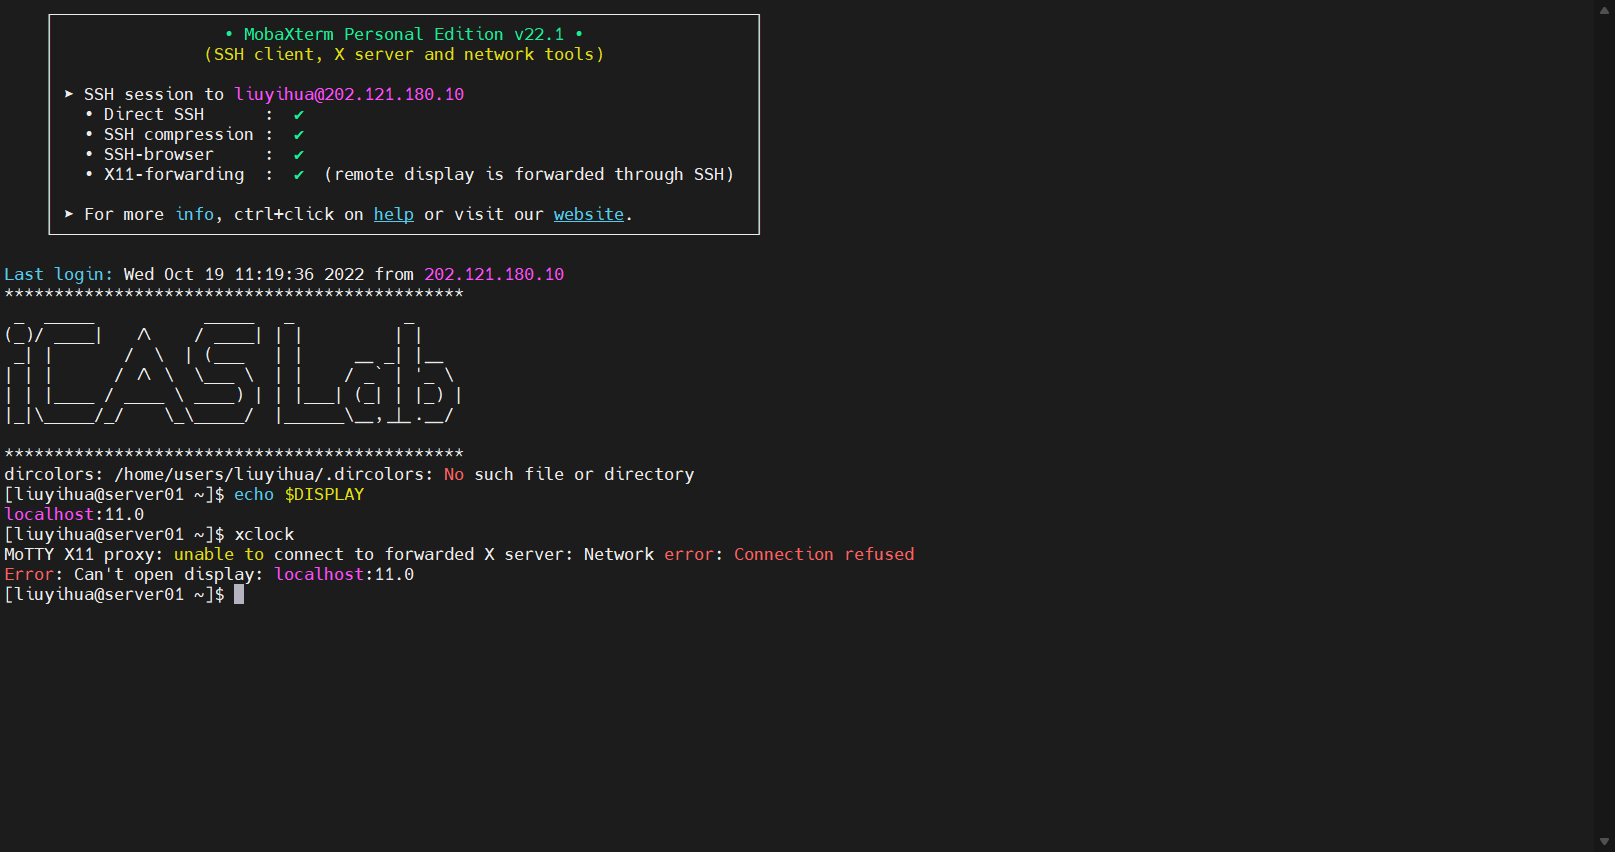
\includegraphics[width=\textwidth]{images/13.png}
    \caption{MobaXterm X11 error.}
\end{figure}
Close all your proxy or VPN connections and restart your computer. Remember that avoid opening any proxy or VPN connections before your launch MobaXterm \cite{uppmax}.
\subsection{OpenLane Make Volare Connection Error}\label{ATVolare}
Please read the reference \cite{volare}. Please just use the SJTU educational network during the setup. If you use other proxy or VPN networks, there are probably problems.

\section{Change Log}
Fall 2022: Yihua Liu
\begin{itemize}
    \item merged, simplified, and updated Lab 6 of Fall 2021 as Section 6
    \item created this lab
\end{itemize}
Fall 2021: Prof. Xinfei Guo
\begin{itemize}
    \item created Lab 6
\end{itemize}

\printbibliography
\end{document}
